\chapter{Resultados y discusión}
\label{chapter:resultados_discusion}

En este capítulo se presentan los resultados obtenidos por el pipeline descrito en el Capítulo~\ref{chapter:metodologia_pipeline}. Primero se reportan las métricas del modelo principal evaluado sobre el conjunto de test independiente. A continuación se presentan los resultados del estudio de ablaciones, la comparación con el baseline lineal (PCA), la comparación con features crudos de FC (sin reducción de dimensionalidad), una comparación entre familias de regresores, el análisis del entrenamiento exclusivo en controles sanos y el impacto de variables demográficas ---tanto como correlatos de la brain age gap como en su rol de features adicionales para la predicción---. Finalmente, se discuten los hallazgos en el contexto de la literatura existente y se identifican las principales limitaciones del trabajo.


\section{Calidad de reconstrucción del $\beta$-VAE}
\label{sec:res_vae}

Antes de evaluar la predicción de edad, es relevante verificar que el $\beta$-VAE aprendió representaciones latentes informativas. La Tabla~\ref{tab:vae_recon} resume las métricas de reconstrucción del modelo final entrenado sobre el conjunto trainval ($n = 1120$).

\begin{table}[H]
\centering
\caption{Métricas de reconstrucción del $\beta$-VAE final sobre el conjunto trainval. Las métricas se reportan como promedio sobre todos los sujetos.}
\label{tab:vae_recon}
\begin{tabular}{lr}
\toprule
\textbf{Métrica} & \textbf{Valor} \\
\midrule
Correlación de Pearson promedio & 0,79 \\
Similitud coseno promedio & 0,87 \\
MAE por feature & 0,124 \\
\bottomrule
\end{tabular}
\end{table}

Una correlación de Pearson de 0,79 indica que la estructura lineal de las matrices de conectividad funcional se preserva en buena medida tras la compresión de 6670 a 64 dimensiones (una reducción del 99\%). La similitud coseno de 0,87 confirma que la dirección general de los vectores se mantiene. Estos valores sugieren que los embeddings capturan información relevante de la conectividad funcional, proporcionando una base adecuada para la etapa de predicción.

La Figura~\ref{fig:vae_recons} muestra tres ejemplos representativos de reconstrucciones del $\beta$-VAE, comparando las matrices de conectividad funcional originales con las reconstruidas a partir del espacio latente. Se puede observar que los patrones globales de conectividad se preservan, aunque los detalles de conexiones individuales presentan cierto suavizado, consistente con la compresión a 64 dimensiones.

\begin{figure}[H]
    \centering
    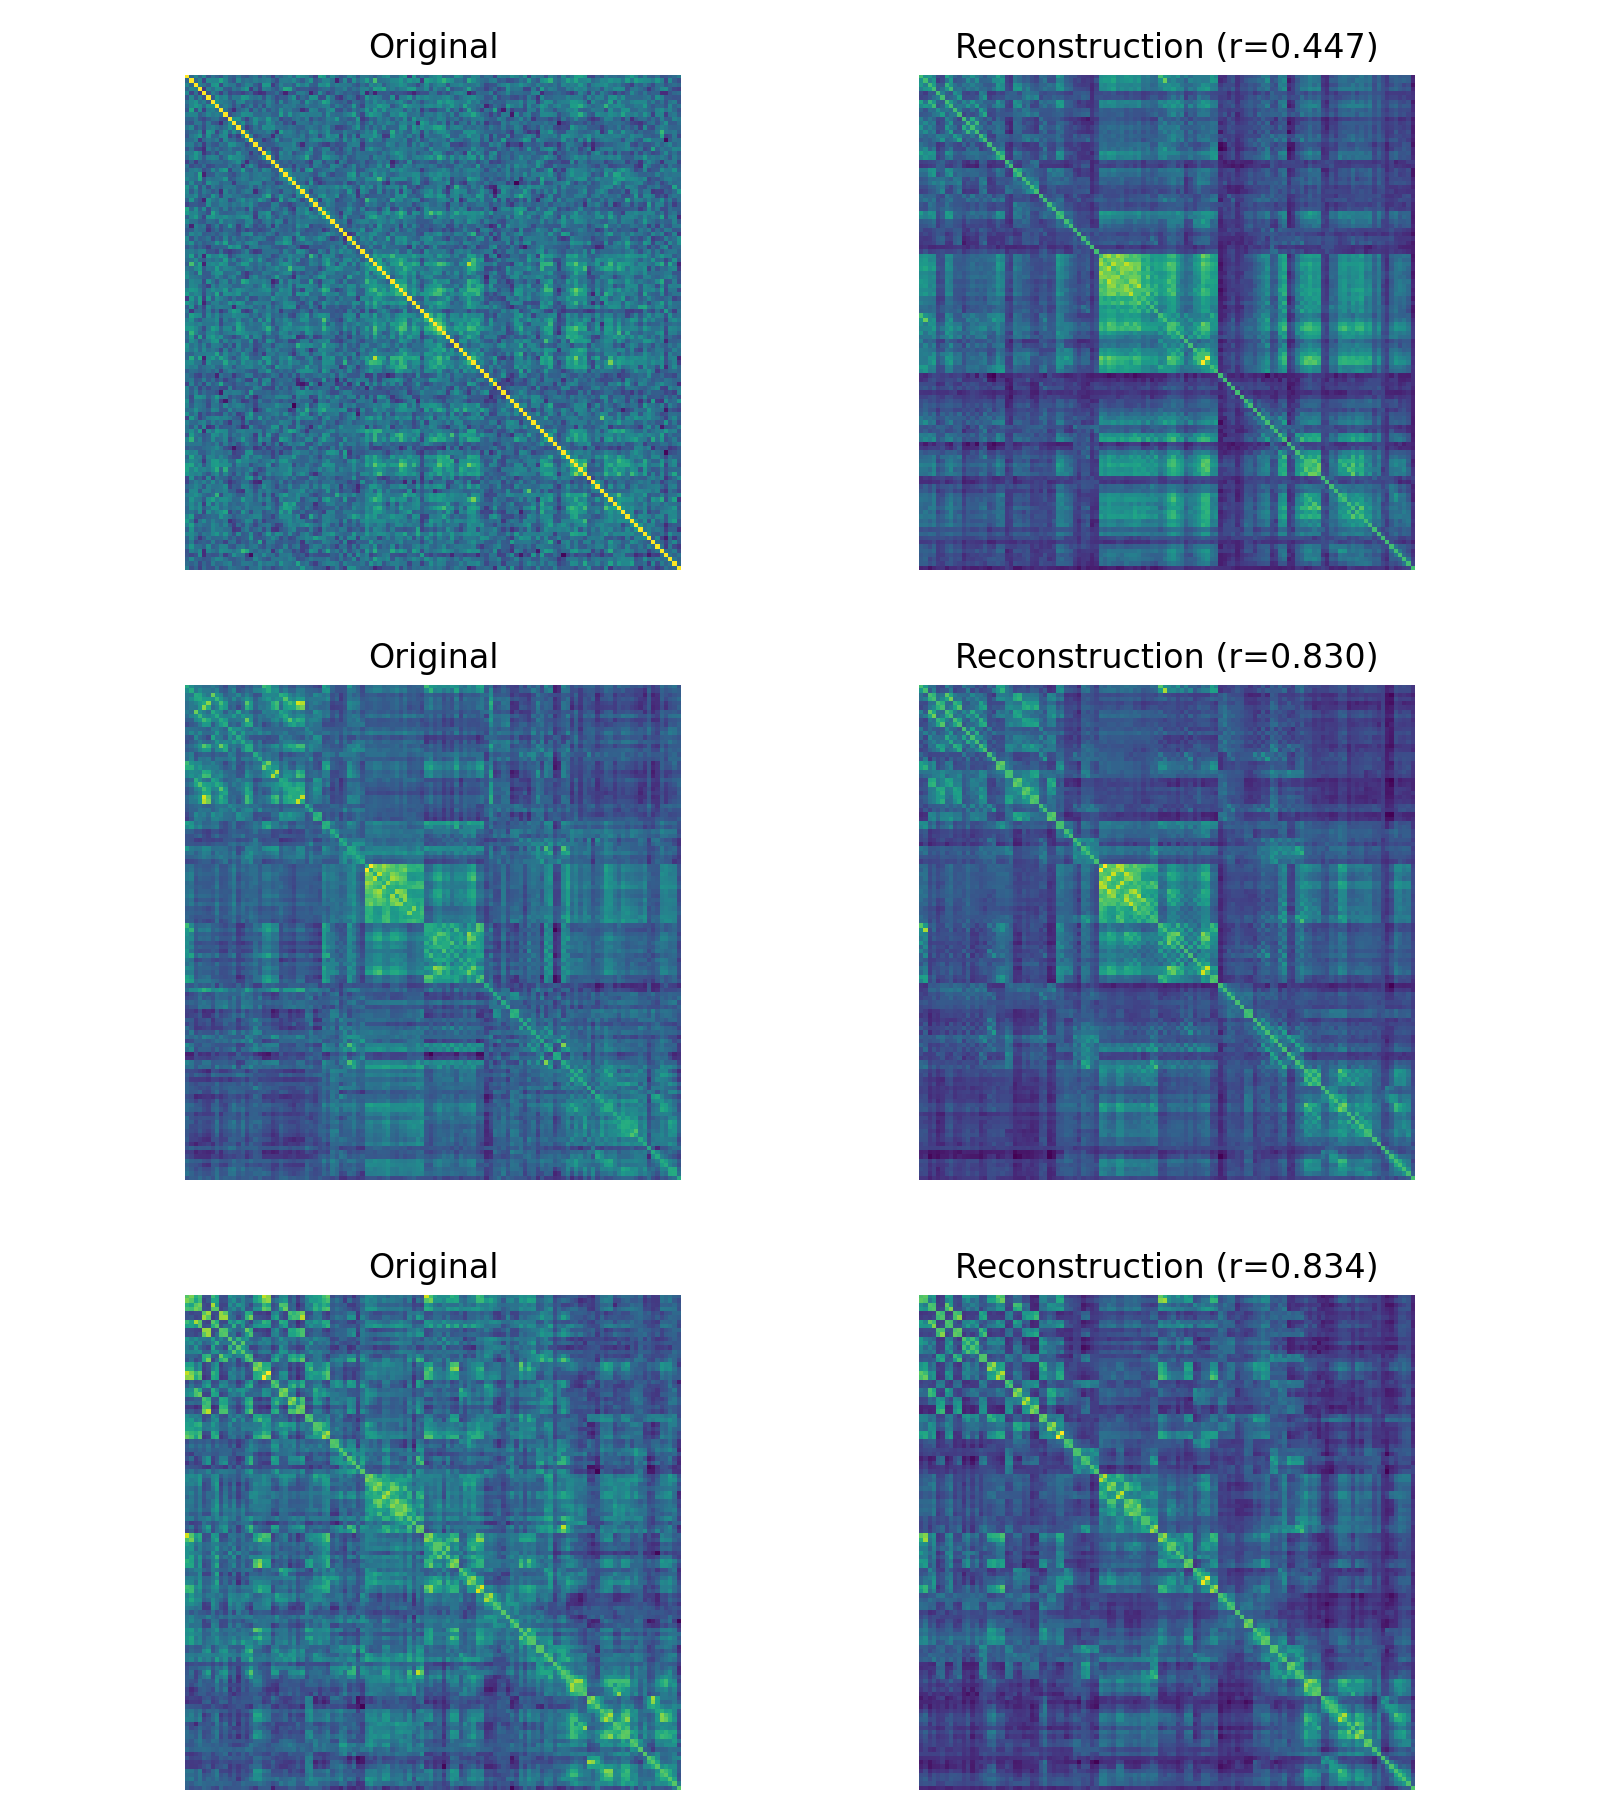
\includegraphics[width=0.85\textwidth]{06_resultados_discusion/images/vae_recons_combined.png}
    \caption{Ejemplos de reconstrucción del $\beta$-VAE para tres sujetos del conjunto trainval. Izquierda: matriz de conectividad funcional original. Derecha: reconstrucción a partir del espacio latente de 64 dimensiones. El valor $r$ indica la correlación de Pearson entre el vector original y el reconstruido para cada sujeto.}
    \label{fig:vae_recons}
\end{figure}


\section{Rendimiento del modelo principal}
\label{sec:res_principal}

El modelo principal (embeddings VAE + features T1w) se evaluó sobre el conjunto de test holdout ($n = 125$), que no fue utilizado durante el entrenamiento ni la selección de hiperparámetros. La Tabla~\ref{tab:test_metrics} presenta las métricas obtenidas.

\begin{table}[H]
\centering
\caption{Métricas de predicción de edad del modelo principal (VAE + T1w) en el conjunto de test ($n = 125$).}
\label{tab:test_metrics}
\begin{tabular}{lr}
\toprule
\textbf{Métrica} & \textbf{Valor} \\
\midrule
MAE & 5,62 años \\
RMSE & 7,20 años \\
$R^2$ & 0,411 \\
Pearson $r$ & 0,644 \\
\bottomrule
\end{tabular}
\end{table}

El modelo logra un error absoluto medio de 5,62 años, lo que significa que en promedio las predicciones se desvían menos de 6 años de la edad cronológica. El $R^2$ de 0,411 indica que el modelo logra dar cuenta de aproximadamente el 41\% de las diferencias de edad entre los sujetos del test; el 59\% restante corresponde a variabilidad que el modelo no captura (diferencias biológicas individuales, ruido de medición, etc.). La correlación de Pearson de 0,644 refleja una asociación moderada-fuerte entre edades reales y predichas. La diferencia entre MAE (5,62) y RMSE (7,20) sugiere la presencia de algunos errores de mayor magnitud en sujetos individuales.

La Figura~\ref{fig:scatter_pred} muestra el diagrama de dispersión entre la edad cronológica y la edad predicha. Los puntos se distribuyen a lo largo de la diagonal de identidad, con una dispersión mayor en los extremos del rango etario, donde la cantidad de sujetos es menor.

\begin{figure}[H]
\centering
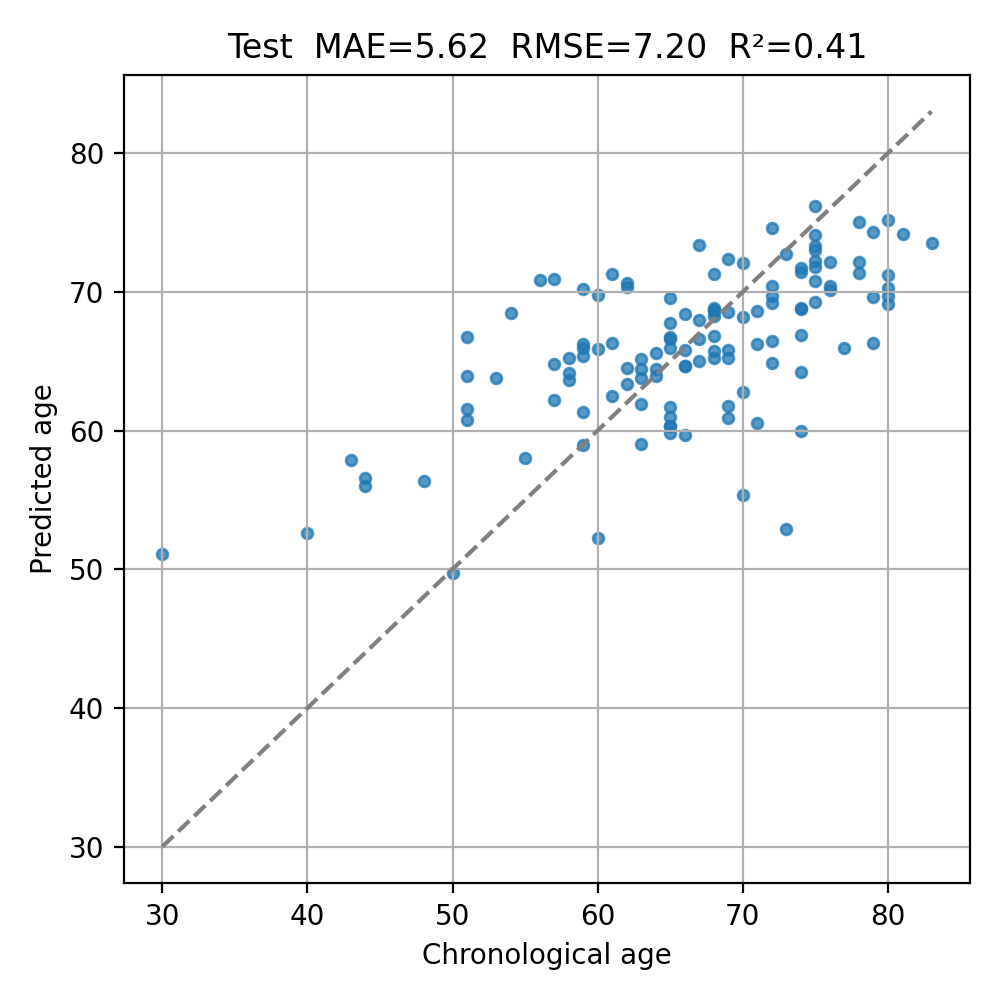
\includegraphics[width=0.7\textwidth]{06_resultados_discusion/images/xgb_scatter.png}
\caption{Edad cronológica vs.\ edad predicha por el modelo principal (VAE + T1w + XGBoost) sobre el conjunto de test ($n = 125$). La línea punteada representa la identidad (predicción perfecta).}
\label{fig:scatter_pred}
\end{figure}

XGBoost proporciona de forma directa una medida de importancia por variable (en este trabajo se usa la métrica Gain, que refleja cuánto reduce cada feature la pérdida cuando se usa en los splits de los árboles). La Figura~\ref{fig:importance} muestra las 20 más influyentes. En el modelo predominan volúmenes de materia gris en cerebelo, cíngulo, corteza frontal, pallidum, lóbulo temporal, hipocampo y tálamo; en la literatura de neuroimagen suelen reportarse cambios en estas estructuras con la edad \cite{raz2005regional, fjell2010structural}, lo que da una interpretabilidad biológica al resultado sin análisis adicionales.

\begin{figure}[H]
\centering
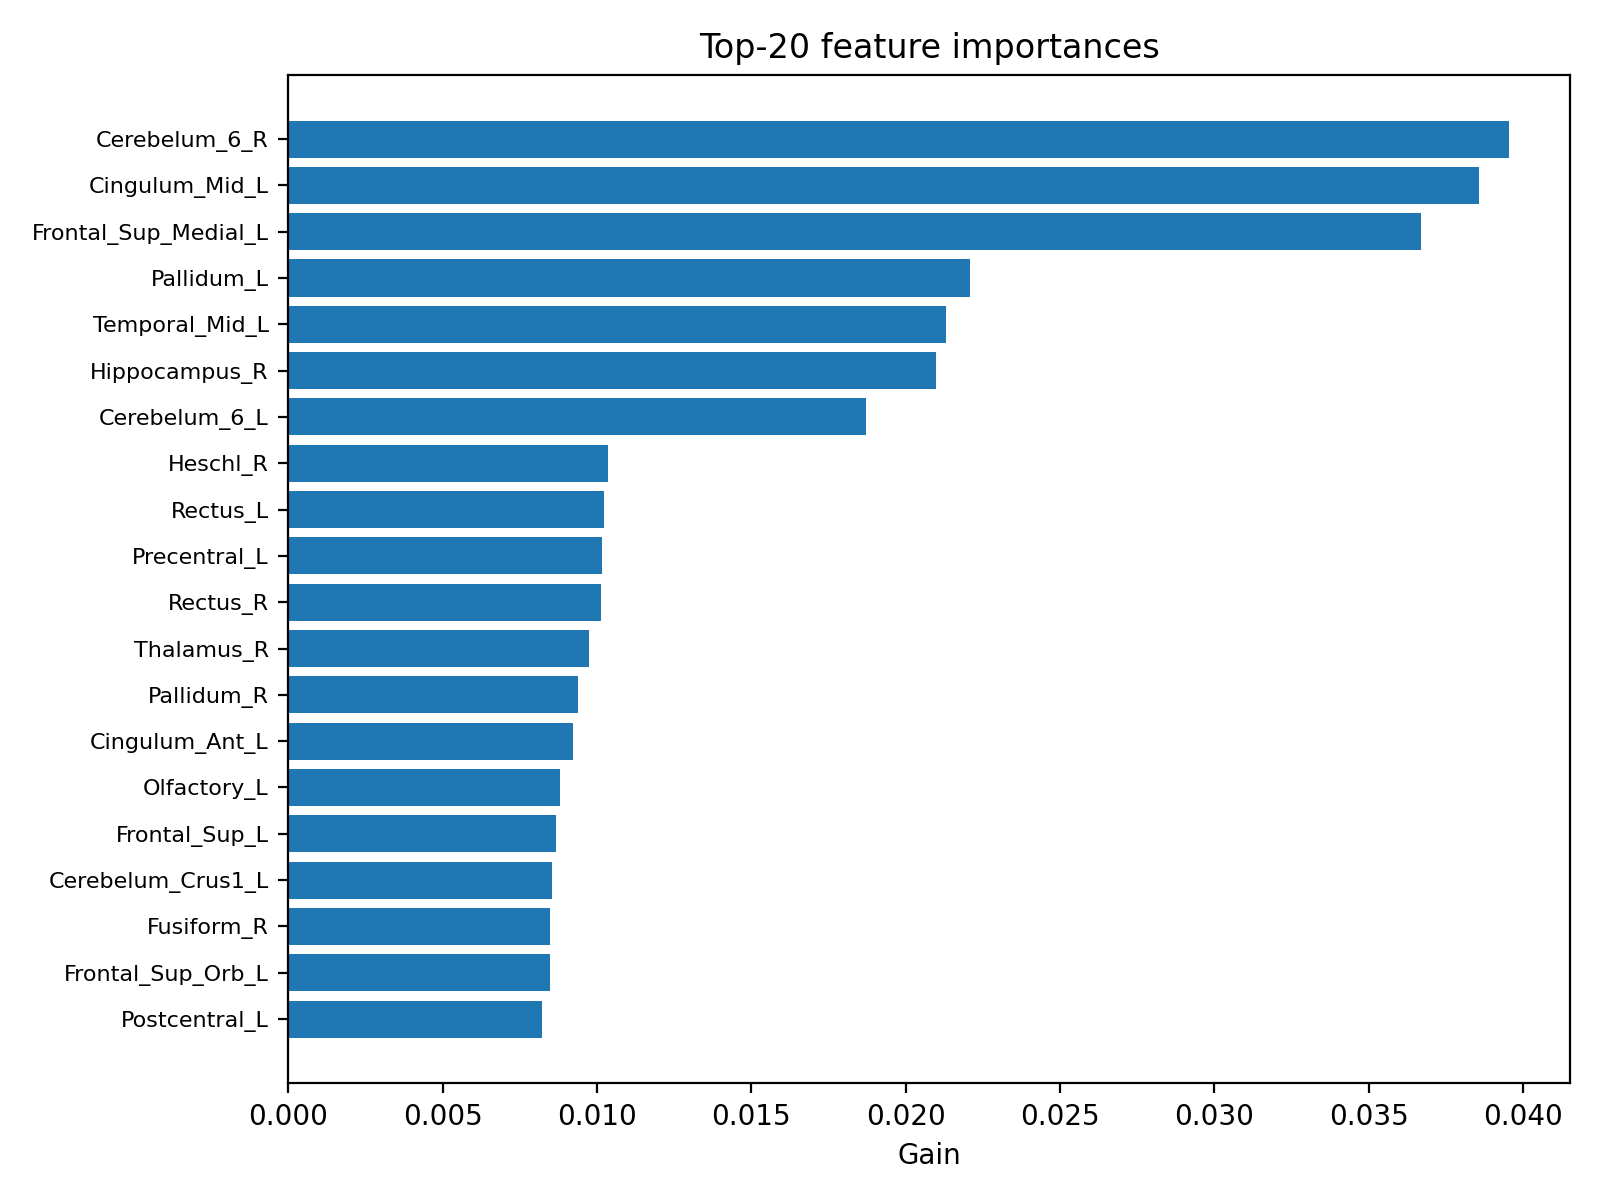
\includegraphics[width=0.85\textwidth]{06_resultados_discusion/images/xgb_importance_top20.png}
\caption{Las 20 features con mayor importancia (Gain) en el modelo XGBoost del pipeline principal. Cada feature T1w tiene la forma \texttt{t1\_XXXX}, donde el número indica el índice de la región en el atlas AAL-116 (orden canónico del atlas); en la figura se muestran los nombres anatómicos correspondientes (p.\ ej.\ Cerebellum\_6\_R, Cingulum\_Mid\_L). Las que más contribuyen coinciden con estructuras asociadas al envejecimiento cerebral en la literatura.}
\label{fig:importance}
\end{figure}


\section{Estudio de ablaciones}
\label{sec:res_ablaciones}

Para cuantificar la contribución de cada fuente de datos, se evaluaron siete configuraciones del modelo sobre el mismo conjunto de test. Todas utilizan los mismos hiperparámetros de XGBoost optimizados, variando únicamente el conjunto de features de entrada. Los resultados se presentan en la Tabla~\ref{tab:ablaciones}.

\begin{table}[H]
\centering
\caption{Resultados del estudio de ablaciones sobre el conjunto de test ($n = 125$). Se resalta en negrita la configuración con mejor MAE.}
\label{tab:ablaciones}
\begin{tabular}{lrrrr}
\toprule
\textbf{Configuración} & \textbf{MAE} & \textbf{RMSE} & \textbf{$R^2$} & \textbf{Pearson} \\
\midrule
Solo T1w & 5,89 & 7,48 & 0,366 & 0,606 \\
T1w + sexo & 5,88 & 7,44 & 0,372 & 0,612 \\
Solo VAE($\mu$) & 7,01 & 9,12 & 0,056 & 0,284 \\
VAE($\mu$) + sexo & 7,06 & 9,18 & 0,044 & 0,268 \\
\textbf{VAE($\mu$) + T1w} & \textbf{5,62} & \textbf{7,20} & \textbf{0,411} & \textbf{0,644} \\
VAE($\mu$) + T1w + sexo & 5,70 & 7,34 & 0,389 & 0,626 \\
VAE($\mu$) + T1w + sexo + diag. & 5,64 & 7,17 & 0,416 & 0,648 \\
\bottomrule
\end{tabular}
\end{table}

El resultado más relevante de las ablaciones es que la configuración VAE + T1w (MAE = 5,62) supera a T1w solo (MAE = 5,89), lo que confirma que los embeddings del VAE capturan patrones de envejecimiento en la conectividad funcional que los volúmenes de materia gris no contienen. La mejora de 0,27 años en MAE y 0,045 puntos en $R^2$ se observa de forma consistente en todas las métricas.

Sin embargo, los embeddings del VAE por sí solos resultan insuficientes: con solo features funcionales, el modelo obtiene un MAE de 7,01 y un $R^2$ de apenas 0,056. La conectividad funcional parece ser una fuente de información más ruidosa que los datos estructurales, y se beneficia sustancialmente de la complementación con T1w.

Resulta llamativo que agregar la variable sexo al modelo no mejore la predicción (MAE 5,70 vs.\ 5,62 sin sexo), a pesar de las diferencias neuroanatómicas documentadas entre sexos. Esto probablemente se deba al tamaño reducido de la muestra, que dificulta capturar efectos sutiles.

En cuanto al diagnóstico, su inclusión produce el mejor $R^2$ (0,416) pero no el mejor MAE (5,64 vs.\ 5,62). Dado que el diagnóstico está correlacionado con la edad (los pacientes con AD tienden a ser mayores), existe el riesgo de que el modelo aprenda un atajo (predecir edad alta para sujetos con AD) en lugar de capturar patrones cerebrales de envejecimiento. Por esta razón se lo excluye del modelo final.


\section{Comparación con reducción lineal (PCA)}
\label{sec:res_pca}

La elección del $\beta$-VAE como método de reducción de dimensionalidad siguió la tendencia predominante en la literatura de neuroimagen computacional, donde los autoencoders variacionales se han consolidado como herramientas estándar para aprender representaciones latentes de datos cerebrales de alta dimensionalidad \cite{higgins2017beta, dufumier2024multi}. No obstante, una vez construido y optimizado el pipeline completo, resulta pertinente validar si la complejidad adicional del VAE respecto a un método lineal clásico se traduce en una mejora de rendimiento. Para ello, se comparó con PCA utilizando 64 componentes (la misma dimensionalidad que el espacio latente del VAE).

Ambos métodos se combinaron con features T1w y se evaluaron con un modelo XGBoost utilizando los hiperparámetros optimizados por Optuna para la configuración VAE + T1w. Dado que ambas configuraciones producen vectores de 180 dimensiones (64 de la reducción + 116 de T1w), estos hiperparámetros son razonables para ambos métodos. Los resultados se presentan en la Tabla~\ref{tab:pca_vs_vae}.

\begin{table}[H]
\centering
\caption{Comparación entre PCA y VAE como método de reducción de dimensionalidad para las matrices de conectividad funcional. Ambos reducen a 64 dimensiones y se combinan con T1w.}
\label{tab:pca_vs_vae}
\begin{tabular}{lrrrr}
\toprule
\textbf{Método} & \textbf{MAE} & \textbf{RMSE} & \textbf{$R^2$} & \textbf{Pearson} \\
\midrule
PCA (64 componentes) & 5,61 & 7,08 & 0,431 & 0,661 \\
$\beta$-VAE (64 dimensiones latentes) & 5,62 & 7,20 & 0,411 & 0,644 \\
\bottomrule
\end{tabular}
\end{table}

Contrariamente a lo esperado, PCA y el $\beta$-VAE alcanzan un rendimiento prácticamente equivalente: la diferencia en MAE es de apenas 0,01 años y en $R^2$ de 0,020, ambas dentro del margen de variabilidad del conjunto de test ($n = 125$). PCA incluso obtiene valores numéricamente superiores en todas las métricas, aunque las diferencias no son estadísticamente significativas. Cabe notar que los hiperparámetros de XGBoost fueron optimizados por Optuna específicamente para la configuración VAE + T1w; si PCA contara con su propia optimización independiente, su rendimiento podría ser incluso superior. En este sentido, el hecho de que PCA iguale o supere al VAE utilizando hiperparámetros ajustados para el VAE refuerza la robustez de este hallazgo.

Este resultado tiene varias implicaciones. Primero, sugiere que la información relevante para la predicción de edad en las matrices de conectividad funcional es capturada en buena medida por las componentes principales, es decir, por las direcciones de máxima varianza. Este hallazgo es consistente con Monti et al. \cite{monti2020interpretable}, quienes demostraron que un enfoque en dos etapas (reducción lineal de dimensionalidad de matrices de conectividad funcional seguida de regresión) permite predecir la edad cerebral de forma generalizable a través de múltiples cohortes. Cabe notar que en ese trabajo, PCA sin restricciones fue el método de menor rendimiento entre los evaluados, y extensiones con restricciones de no-negatividad y ortogonalidad obtuvieron mejores resultados; sin embargo, en el presente trabajo el uso de un regresor no lineal (XGBoost) en la segunda etapa podría compensar la simplicidad de PCA en la primera. Segundo, indica que un regresor suficientemente potente como XGBoost puede extraer patrones no lineales incluso a partir de features linealmente proyectados, lo que reduce la ventaja de una representación no lineal como la del VAE. Tercero, la convergencia de resultados entre PCA y VAE es consistente con el hallazgo de la Sección~\ref{sec:res_regresores}, donde tres familias de regresores diferentes también alcanzan rendimientos equivalentes: una vez que los datos se comprimen a una dimensionalidad adecuada, el rendimiento depende más de la información contenida en los datos que del método de representación o del regresor. More et al. \cite{more2023brain}, en su comparación sistemática de 128 workflows de predicción de brain age, observaron que tanto la representación de los datos como el algoritmo de aprendizaje automático afectan el rendimiento, y que las features a nivel de vóxel combinadas con PCA y algoritmos no lineales se encuentran entre las configuraciones de mejor desempeño.

No obstante, este resultado debe interpretarse con cautela. La optimización de la arquitectura del VAE exploró únicamente 70 configuraciones (trials de Optuna) dentro de un espacio de búsqueda combinatorio vasto que incluye la dimensión latente, el número y tamaño de capas ocultas, el valor de $\beta$, la tasa de dropout, el learning rate, las épocas de warmup y el tipo de embedding. Es plausible que configuraciones no exploradas del VAE logren un rendimiento superior al de PCA, particularmente con cohortes mayores donde los métodos no lineales suelen beneficiarse de la mayor cantidad de datos de entrenamiento.

Además, el $\beta$-VAE ofrece ventajas cualitativas que PCA no posee y que justifican su inclusión en el pipeline. Como modelo generativo, permite la reconstrucción y visualización de las matrices FC originales a partir del espacio latente, proporcionando una herramienta de verificación de la calidad de las representaciones aprendidas. Asimismo, la optimización downstream de sus hiperparámetros orienta la representación hacia la tarea de predicción de edad, una capacidad que PCA no puede ofrecer (carece de hiperparámetros ajustables más allá del número de componentes).


\section{Comparación con features crudos de FC (sin reducción)}
\label{sec:res_raw_fc}

Para evaluar si la reducción de dimensionalidad del VAE es realmente necesaria, o si XGBoost puede manejar directamente los features de alta dimensionalidad, se comparó el pipeline VAE + T1w con una variante que utiliza los 6670 valores crudos del triángulo superior de la matriz FC concatenados con los 116 features T1w (6786 features totales). Para garantizar una comparación justa, los hiperparámetros de XGBoost se optimizaron de forma independiente con Optuna (50 trials, 5-fold CV) para cada configuración, en lugar de reutilizar los parámetros optimizados para una de las dos. Los resultados se presentan en la Tabla~\ref{tab:raw_fc_vs_vae}.

\begin{table}[H]
\centering
\caption{Comparación entre el uso directo de los features crudos de FC y la reducción vía $\beta$-VAE, ambos combinados con T1w. Cada configuración tiene hiperparámetros de XGBoost optimizados independientemente con Optuna.}
\label{tab:raw_fc_vs_vae}
\begin{tabular}{lrrrrr}
\toprule
\textbf{Método} & \textbf{Features} & \textbf{MAE} & \textbf{RMSE} & \textbf{$R^2$} & \textbf{Pearson} \\
\midrule
FC crudo + T1w & 6786 & 6,00 & 7,55 & 0,354 & 0,601 \\
$\beta$-VAE + T1w & 180 & 5,62 & 7,20 & 0,411 & 0,644 \\
\midrule
\textbf{Ventaja del VAE} & \textbf{$-$97,3\%} & \textbf{$-$0,38} & \textbf{$-$0,35} & \textbf{+0,057} & \textbf{+0,043} \\
\bottomrule
\end{tabular}
\end{table}

Aun con hiperparámetros optimizados específicamente para la entrada de alta dimensionalidad, el VAE supera a los features crudos en todas las métricas: la mejora en MAE es de 0,38 años y en $R^2$ de 16\% relativo (de 0,354 a 0,411). La correlación de Pearson también es superior (0,644 vs.\ 0,601). Esto confirma que la ventaja del VAE no se debe a una elección desfavorable de hiperparámetros, sino a la calidad de las representaciones aprendidas.

El análisis de los hiperparámetros optimizados por Optuna para cada configuración es revelador. Para el pipeline VAE + T1w (180 features), Optuna seleccionó árboles profundos (\texttt{max\_depth}~$= 6$) que observan casi todas las features por árbol. En cambio, para los features crudos (6786), Optuna seleccionó árboles poco profundos (\texttt{max\_depth}~$= 3$) donde cada árbol observa solo el 10\% de los features, con mayor regularización y un peso mínimo por hoja diez veces superior. Esto indica que el regresor necesita una regularización agresiva para manejar la alta dimensionalidad, descartando implícitamente la mayoría de los features en cada paso. La compresión del VAE realiza esta selección de información de forma más sistemática y efectiva, produciendo representaciones densas donde todas las dimensiones son informativas.


\section{Comparación de regresores}
\label{sec:res_regresores}

Para evaluar si el rendimiento del pipeline depende del regresor específico o de la representación aprendida, se compararon tres familias de modelos: regresión lineal regularizada (Ridge), regresión por vectores de soporte con kernel RBF (SVR) y gradient boosting (XGBoost). Los tres regresores recibieron exactamente las mismas features de entrada (embeddings VAE $\mu$ + T1w, 180 dimensiones) y se evaluaron sobre los mismos conjuntos de validación cruzada y test.

Para garantizar una comparación justa, los hiperparámetros de cada modelo se optimizaron con Optuna mediante 100 trials sobre los mismos 5 folds de validación cruzada empleados en el pipeline principal. Los resultados se resumen en la Tabla~\ref{tab:model_comparison}.

\begin{table}[H]
\centering
\caption{Comparación de regresores, todos optimizados con Optuna (100 trials, 5-fold CV). Se reportan el MAE de validación cruzada (CV MAE) y las métricas sobre el conjunto de test ($n = 125$).}
\label{tab:model_comparison}
\begin{tabular}{lrrrrr}
\toprule
\textbf{Modelo} & \textbf{CV MAE} & \textbf{MAE} & \textbf{RMSE} & \textbf{$R^2$} & \textbf{Pearson} \\
\midrule
Ridge          & 6,54 & 5,75 & 7,25 & 0,403 & 0,639 \\
SVR (RBF)      & 6,22 & 5,65 & 7,02 & 0,441 & 0,664 \\
XGBoost        & 6,36 & 5,62 & 7,20 & 0,411 & 0,644 \\
\bottomrule
\end{tabular}
\end{table}

Los tres regresores alcanzan un rendimiento muy similar: la diferencia máxima en MAE de test es de apenas 0,13 años entre Ridge y XGBoost, y de 0,03 años entre SVR y XGBoost. En validación cruzada, SVR obtiene el menor error promedio (6,22), mientras que XGBoost presenta el menor MAE de test (5,62). Estas diferencias se encuentran dentro del margen de variabilidad esperado para un conjunto de test de 125 sujetos.

La convergencia de rendimiento entre tres familias de modelos fundamentalmente distintas (lineal, kernel y ensemble de árboles) indica que el factor determinante de la predicción no es el regresor sino la calidad de las representaciones construidas en la etapa de extracción de features. Se mantiene XGBoost en el pipeline principal por una razón práctica de interpretación: los árboles de decisión permiten obtener, del propio entrenamiento, una medida de importancia por variable (Gain), sin necesidad de análisis adicionales. Con Ridge solo se tienen coeficientes de una combinación lineal, y con SVR la interpretación de la contribución individual de cada feature resulta considerablemente más compleja. Con XGBoost basta con consultar las importancias nativas del modelo para discutir qué regiones o dimensiones latentes son más relevantes (Figura~\ref{fig:importance}).


\section{Evaluación del entrenamiento exclusivo en controles sanos}
\label{sec:res_cn_only}

Se evaluó una estrategia alternativa en la que tanto el VAE como el XGBoost se entrenan exclusivamente sobre los sujetos cognitivamente normales (CN) del conjunto trainval ($n_{\text{CN}} = 473$), con el objetivo de aprender el patrón de envejecimiento normal y medir la \textit{brain age gap} en poblaciones clínicas.

Dado que el modelo fue entrenado únicamente con sujetos CN, todos los pacientes con AD y FTD constituyen datos no vistos durante el entrenamiento. Esto permite utilizar la totalidad de ambos grupos clínicos para la evaluación, no solamente los sujetos del conjunto de test del pipeline principal. En cambio, para los sujetos CN se emplean únicamente los 53 del conjunto de test, ya que los restantes 473 fueron utilizados para entrenar el modelo. Los resultados por grupo diagnóstico se presentan en la Tabla~\ref{tab:cn_only}.

\begin{table}[H]
\centering
\caption{Rendimiento del modelo entrenado exclusivamente en controles sanos. CN se evalúa sobre los 53 sujetos del conjunto de test; AD y FTD se evalúan sobre la totalidad de sus respectivas cohortes, ya que ninguno fue utilizado durante el entrenamiento.}
\label{tab:cn_only}
\begin{tabular}{lrrrrrr}
\toprule
\textbf{Grupo} & \textbf{$n$} & \textbf{MAE} & \textbf{RMSE} & \textbf{$R^2$} & \textbf{Pearson} & \textbf{Gap} \\
\midrule
CN  & 53  & 6,03 & 7,33 & 0,504  & 0,717 & $-$0,42 \\
AD  & 422 & 7,36 & 9,19 & $-$0,170 & 0,129 & $-$1,86 \\
FTD & 297 & 6,93 & 8,90 & $-$0,153 & 0,165 & $+$1,84 \\
\bottomrule
\end{tabular}
\end{table}

El modelo CN-only obtiene un MAE de 6,03 años en los 53 sujetos CN del test, superior al MAE de 5,62 del modelo mixto. Esto indica que, con 473 sujetos sanos, el modelo no captura los patrones del envejecimiento normal con precisión suficiente. En ambas poblaciones clínicas, los valores de $R^2$ son negativos, lo que indica predicciones peores que la media, y las correlaciones de Pearson son débiles ($< 0{,}2$).

La brain age gap media en FTD fue de $+1{,}84$ años, es decir, el modelo predice que los pacientes con demencia frontotemporal tienen cerebros \textit{más viejos} que su edad cronológica. Esta dirección coincide con la esperada en la literatura, donde el envejecimiento acelerado es un marcador de neurodegeneración \cite{franke2010estimating}. Sin embargo, en AD la gap fue de $-1{,}86$ años (dirección opuesta), lo que contradice la evidencia publicada. La divergencia entre ambos grupos clínicos sugiere que, con 473 sujetos de entrenamiento, el modelo captura una señal débil e inconsistente, insuficiente para funcionar como biomarcador.

El rendimiento inferior respecto al modelo mixto podría atribuirse a dos factores: (i)~la reducción del conjunto de entrenamiento (473 sujetos frente a 1120), y (ii)~la reutilización de hiperparámetros optimizados para la cohorte completa, que pueden no ser óptimos para la sub-cohorte CN. Para descartar el factor~(ii), se realizó un experimento adicional con optimización Optuna dedicada para los datos CN (50 trials para el $\beta$-VAE y 100 para XGBoost). Los resultados fueron similares: MAE de 6,29 en CN, gaps de $-2{,}21$ en AD y $+1{,}71$ en FTD, confirmando que la limitación principal es el tamaño de la muestra y no la configuración de hiperparámetros. Esto es consistente con la literatura, donde los estudios de brain age basados exclusivamente en sujetos sanos suelen requerir cohortes del orden de $N > 2000$ para obtener MAE competitivos y gaps clínicamente significativos \cite{franke2010estimating}.

Por estas razones, se descartó este enfoque en favor del entrenamiento mixto (CN + AD + FTD), que obtiene un rendimiento más robusto y generalizable (MAE = 5,62) y aprovecha la totalidad de la muestra disponible.

\subsection{Modelo CN-only con variables demográficas}
\label{sec:res_cn_demo}

De forma exploratoria, se evaluó si la inclusión de variables demográficas (educación y sitio) podría mejorar el modelo CN-only. Para este experimento se utilizaron únicamente los 337 sujetos CN que disponen de datos demográficos completos, lo que constituye una reducción adicional respecto a los 473 CN del experimento anterior. La Tabla~\ref{tab:cn_demo} compara los resultados del modelo CN-only con y sin variables demográficas.

\begin{table}[H]
\centering
\caption{Modelo CN-only con y sin variables demográficas. Ambos modelos fueron entrenados exclusivamente con los 337 CN que disponen de datos demográficos (a diferencia de la Tabla~\ref{tab:cn_only}, que utiliza los 473 CN totales); la diferencia de tamaño y composición del conjunto de entrenamiento explica las diferencias numéricas entre ambas tablas. Los grupos clínicos (AD, FTD) incluyen únicamente los sujetos con datos demográficos disponibles.}
\label{tab:cn_demo}
\begin{tabular}{llrrrr}
\toprule
\textbf{Modelo} & \textbf{Grupo} & \textbf{$n$} & \textbf{MAE} & \textbf{$R^2$} & \textbf{Gap} \\
\midrule
\multirow{3}{*}{CN baseline} & CN (test) & 53 & 6,09 & 0,487 & $-$0,07 \\
                             & AD       & 422 & 6,97 & $-$0,113 & $+$0,21 \\
                             & FTD      & 297 & 7,42 & $-$0,335 & $+$4,01 \\
\midrule
\multirow{3}{*}{CN + edu + sitio} & CN (test) & 37 & 5,51 & 0,569 & $+$0,41 \\
                                  & AD       & 348 & 6,41 & 0,054 & $+$0,70 \\
                                  & FTD      & 211 & 6,49 & $-$0,071 & $+$4,11 \\
\bottomrule
\end{tabular}
\end{table}

La inclusión de educación y sitio mejora el MAE en CN de 6,09 a 5,51 años y, de forma relevante, las gaps en ambos grupos clínicos son consistentemente positivas: $+0{,}70$ en AD y $+4{,}11$ en FTD. Esta dirección (cerebro más viejo de lo esperado) es la esperada en la neurodegeneración. En contraste, el modelo CN baseline sin demográficos obtiene una gap cercana a cero en AD ($+0{,}21$), lo que dificulta la interpretación clínica. La Figura~\ref{fig:cn_demo_importance} muestra la importancia de las features en el modelo CN + educación + sitio: la variable \texttt{education} se posiciona entre las más relevantes, lo que sugiere que la información socioeconómica aporta señal complementaria a las features de neuroimagen.

\begin{figure}[H]
\centering
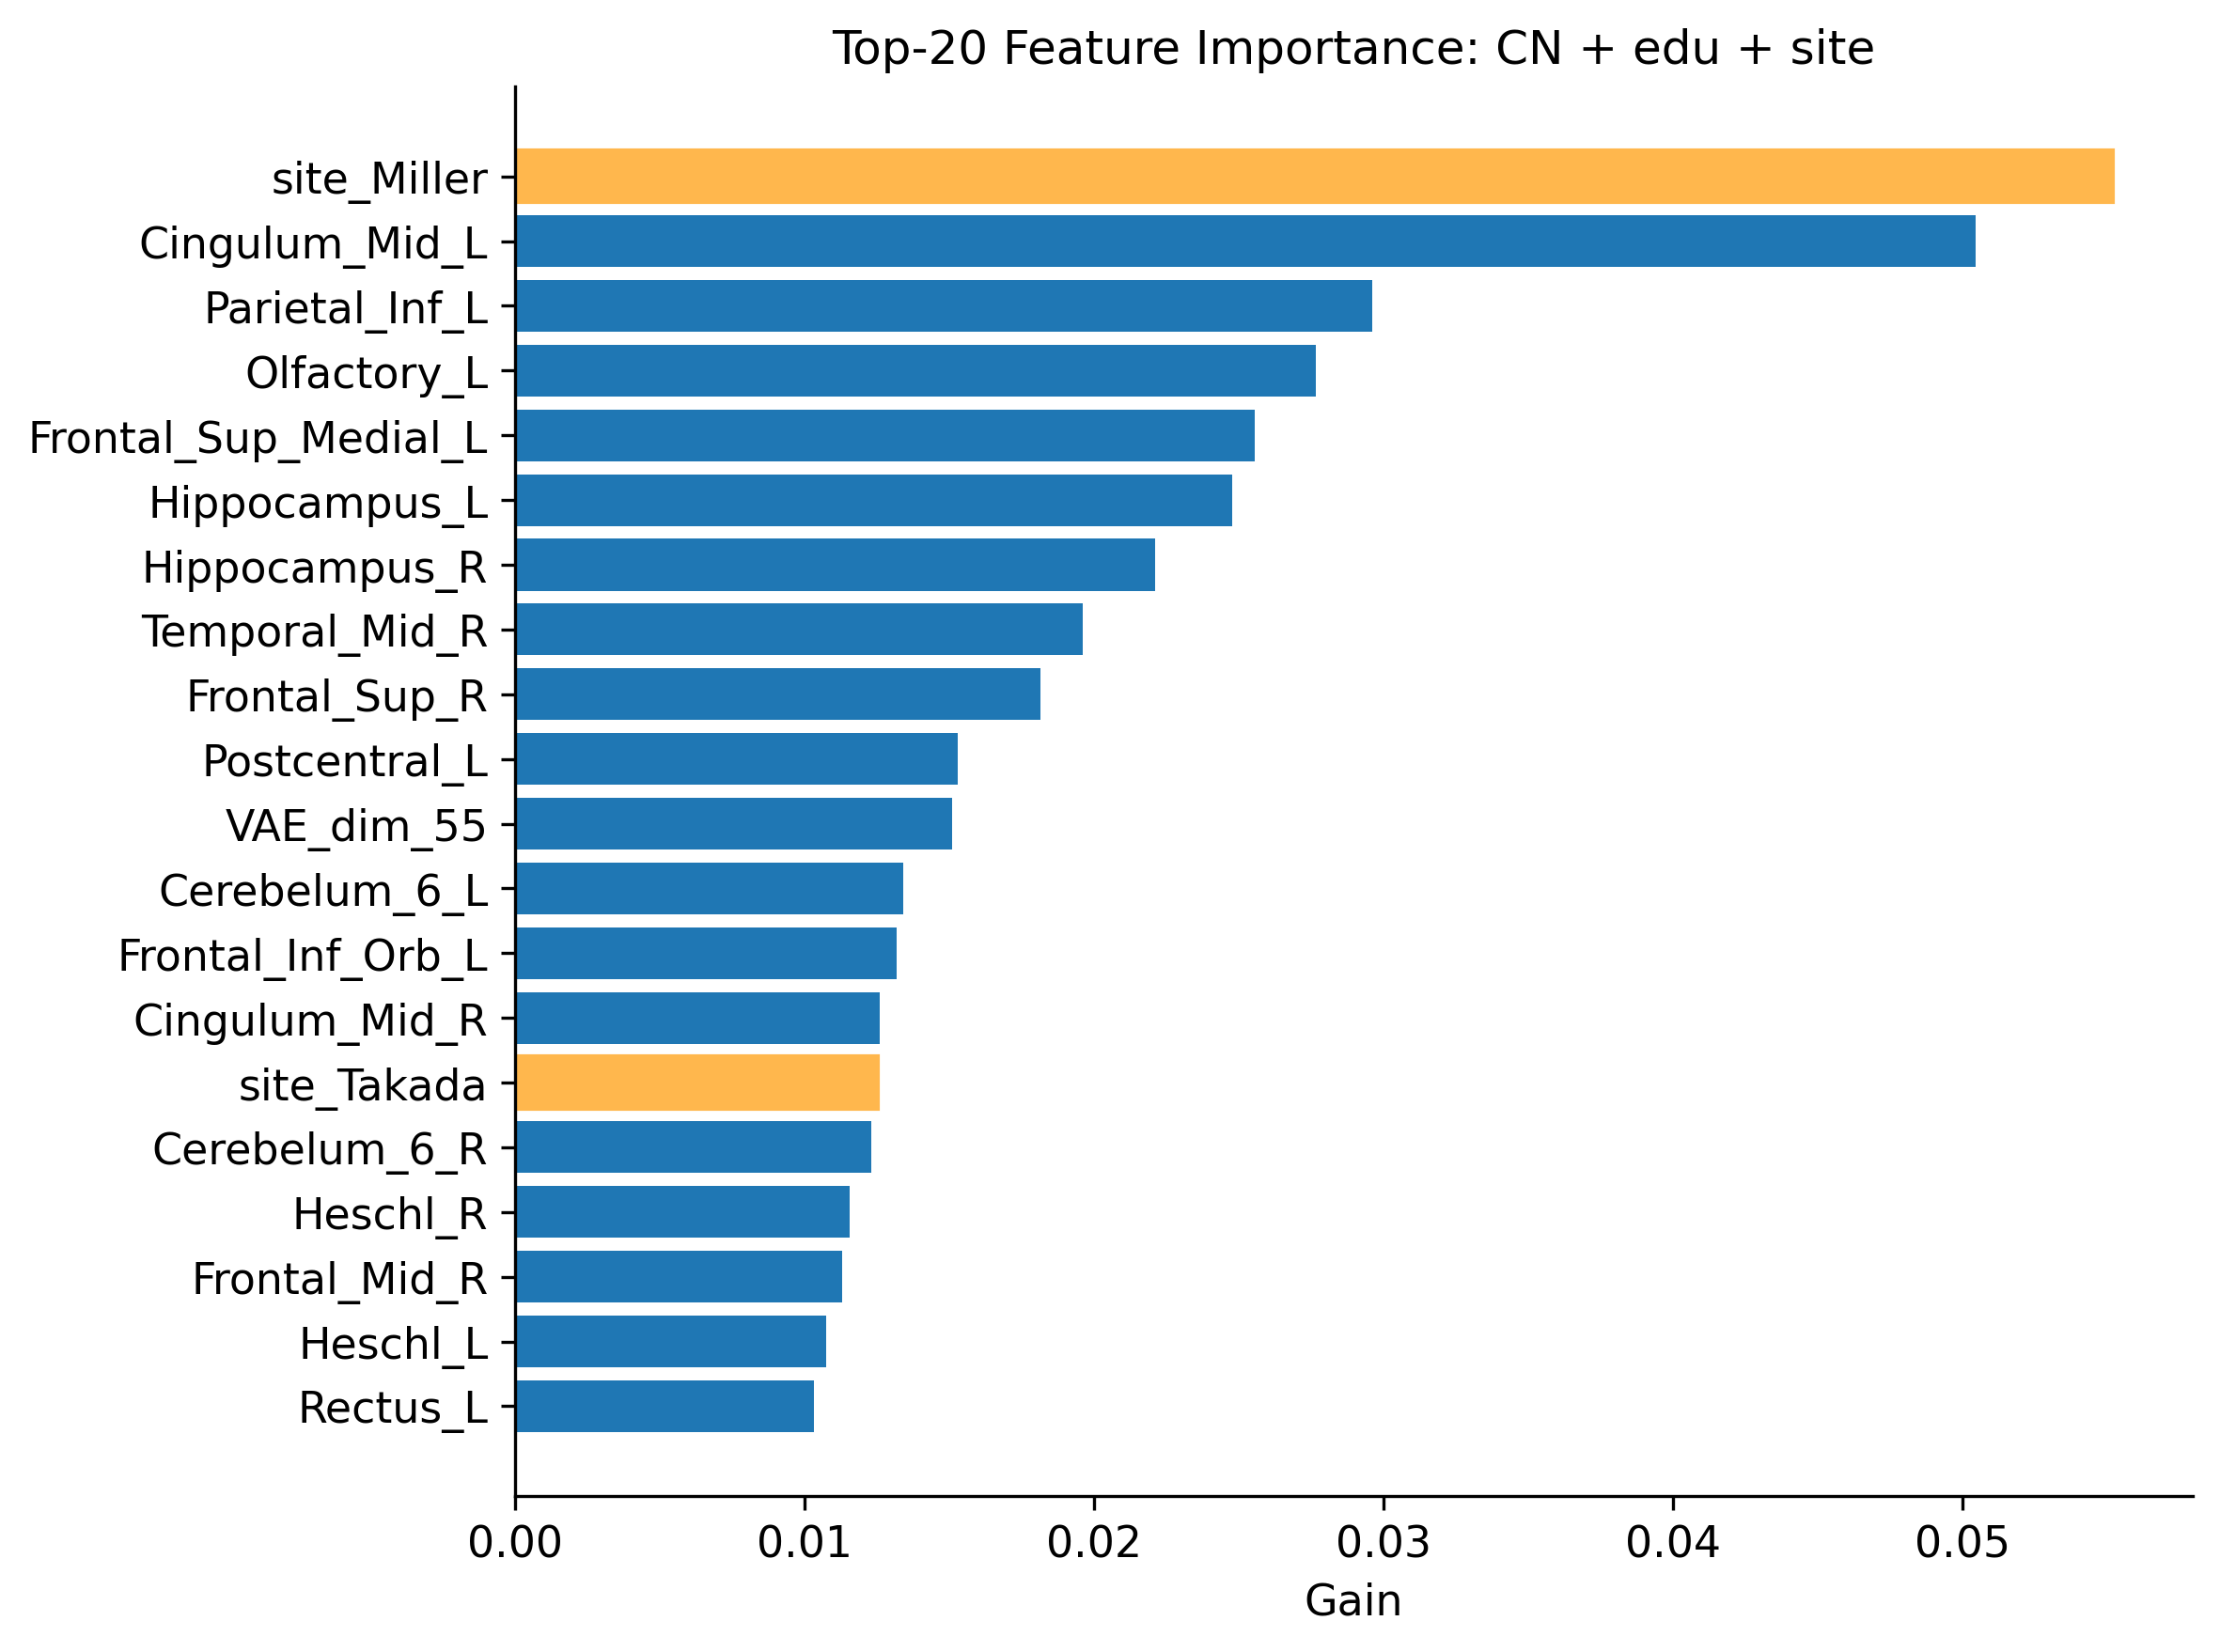
\includegraphics[width=0.7\textwidth]{06_resultados_discusion/images/cn_demo_importance.png}
\caption{Top 20 features por importancia (XGBoost \textit{gain}) en el modelo CN-only entrenado con educación y sitio como features adicionales. Las features VAE\_dim\_$N$ representan dimensiones latentes del $\beta$-VAE (patrones de conectividad funcional) y no corresponden a una región cerebral individual.}
\label{fig:cn_demo_importance}
\end{figure}

Estos resultados son exploratorios y deben interpretarse con cautela dado el reducido tamaño de la muestra de entrenamiento ($n = 337$ CN) y de test ($n = 37$ CN). No obstante, la consistencia de las gaps positivas en ambos grupos clínicos sugiere que, con una cohorte CN más amplia y datos demográficos completos, la inclusión de estas variables podría contribuir a mejorar la viabilidad del pipeline como biomarcador.

\section{Impacto de variables demográficas}
\label{sec:res_demograficas}

Dada la heterogeneidad socioeconómica y multicéntrica de la cohorte RedLaT, se analizó el impacto de variables demográficas sobre la predicción de edad cerebral. Las variables exploradas fueron los años de educación formal (\texttt{cog\_ed}, disponible para el 74,9\% de la cohorte), el sitio de adquisición (75,6\%) y la marca del escáner MRI (74,0\%). El análisis se realizó en dos direcciones complementarias: (i)~correlación entre las variables demográficas y la brain age gap del modelo principal, y (ii)~inclusión de dichas variables como features adicionales en el modelo de predicción.

\subsection{Brain age gap y años de educación}
\label{sec:res_gap_educacion}

Antes de evaluar si las variables demográficas mejoran la predicción del modelo (lo cual se analiza en la Sección~\ref{sec:res_demo_ablacion}), es relevante entender si estas variables se \emph{asocian} con los errores que el modelo ya comete. Para ello se utiliza la brain age gap, es decir, la diferencia entre la edad que el modelo predice para el cerebro de una persona y su edad cronológica real. Por ejemplo, si el modelo dice que el cerebro de una persona de 60 años ``parece'' de 65, su gap es de $+5$ años; si parece de 55, su gap es de $-5$ años. Una gap positiva indica que el modelo percibe un cerebro más envejecido de lo esperado, y una negativa lo contrario.

La pregunta concreta de esta sección es: ¿las personas con más años de educación tienden a tener gaps más positivas o más negativas? Y lo mismo para cada grupo diagnóstico por separado. La respuesta no nos dice si agregar educación al modelo mejora su precisión (eso se responde después), sino si la educación está relacionada con que el modelo sobreestime o subestime la edad cerebral, lo cual tiene implicaciones para entender los factores que modulan el envejecimiento.

Para cada sujeto se calculó la gap a partir de las predicciones del modelo principal. En el caso de los sujetos del conjunto trainval, las predicciones se obtuvieron mediante validación cruzada con 5 folds para evitar el sobreajuste. La Tabla~\ref{tab:gap_education} resume las correlaciones (Pearson $r$ y Spearman $\rho$; véase la Sección~\ref{sec:analisis_exploratorio} del Capítulo~\ref{chapter:datos_cohorte} para una explicación detallada de estos coeficientes) entre la gap y los años de educación, estratificadas por diagnóstico.

\begin{table}[H]
\centering
\caption{Correlación entre brain age gap y años de educación, por grupo diagnóstico.}
\label{tab:gap_education}
\begin{tabular}{lrrrrr}
\toprule
\textbf{Grupo} & \textbf{$n$} & \textbf{Pearson $r$} & \textbf{$p$} & \textbf{Spearman $\rho$} & \textbf{$p$} \\
\midrule
CN  & 374 & $-$0,067 & 0,193  & $-$0,091 & 0,079 \\
AD  & 348 & $+$0,165 & 0,002  & $+$0,157 & 0,003 \\
FTD & 211 & $+$0,002 & 0,980  & $-$0,025 & 0,716 \\
Todos & 933 & $+$0,070 & 0,033  & $+$0,038 & 0,251 \\
\bottomrule
\end{tabular}
\end{table}

En controles sanos, la correlación es débil y no significativa ($r = -0{,}067$, $p = 0{,}19$), aunque la dirección negativa sugiere una tendencia sutil en la que mayor educación se asocia con un cerebro predicho como ligeramente más joven. Este patrón es consistente con la hipótesis de reserva cognitiva, que propone que la educación y la estimulación intelectual acumulada a lo largo de la vida fortalecen las redes neuronales, permitiendo al cerebro tolerar mayor daño antes de manifestar síntomas clínicos; en términos del modelo, esto se traduciría en un cerebro que ``aparenta'' ser más joven de lo esperado para su edad cronológica.

En pacientes con AD, la correlación es positiva y estadísticamente significativa ($r = +0{,}165$, $p = 0{,}002$): mayor educación se asocia con una gap más positiva (cerebro predicho como más viejo). Este hallazgo, aparentemente paradójico, puede explicarse por la misma reserva cognitiva: los pacientes con mayor educación mantienen el funcionamiento cognitivo durante más tiempo a pesar de la neurodegeneración, por lo que acceden al diagnóstico en estadios más avanzados de la enfermedad, cuando la atrofia cerebral es más pronunciada y el modelo detecta un cerebro significativamente más envejecido. En FTD no se observa correlación ($r \approx 0$).

La Figura~\ref{fig:demo_gap_vs_education} ilustra la relación entre la brain age gap y los años de educación para cada grupo diagnóstico.

\begin{figure}[H]
\centering
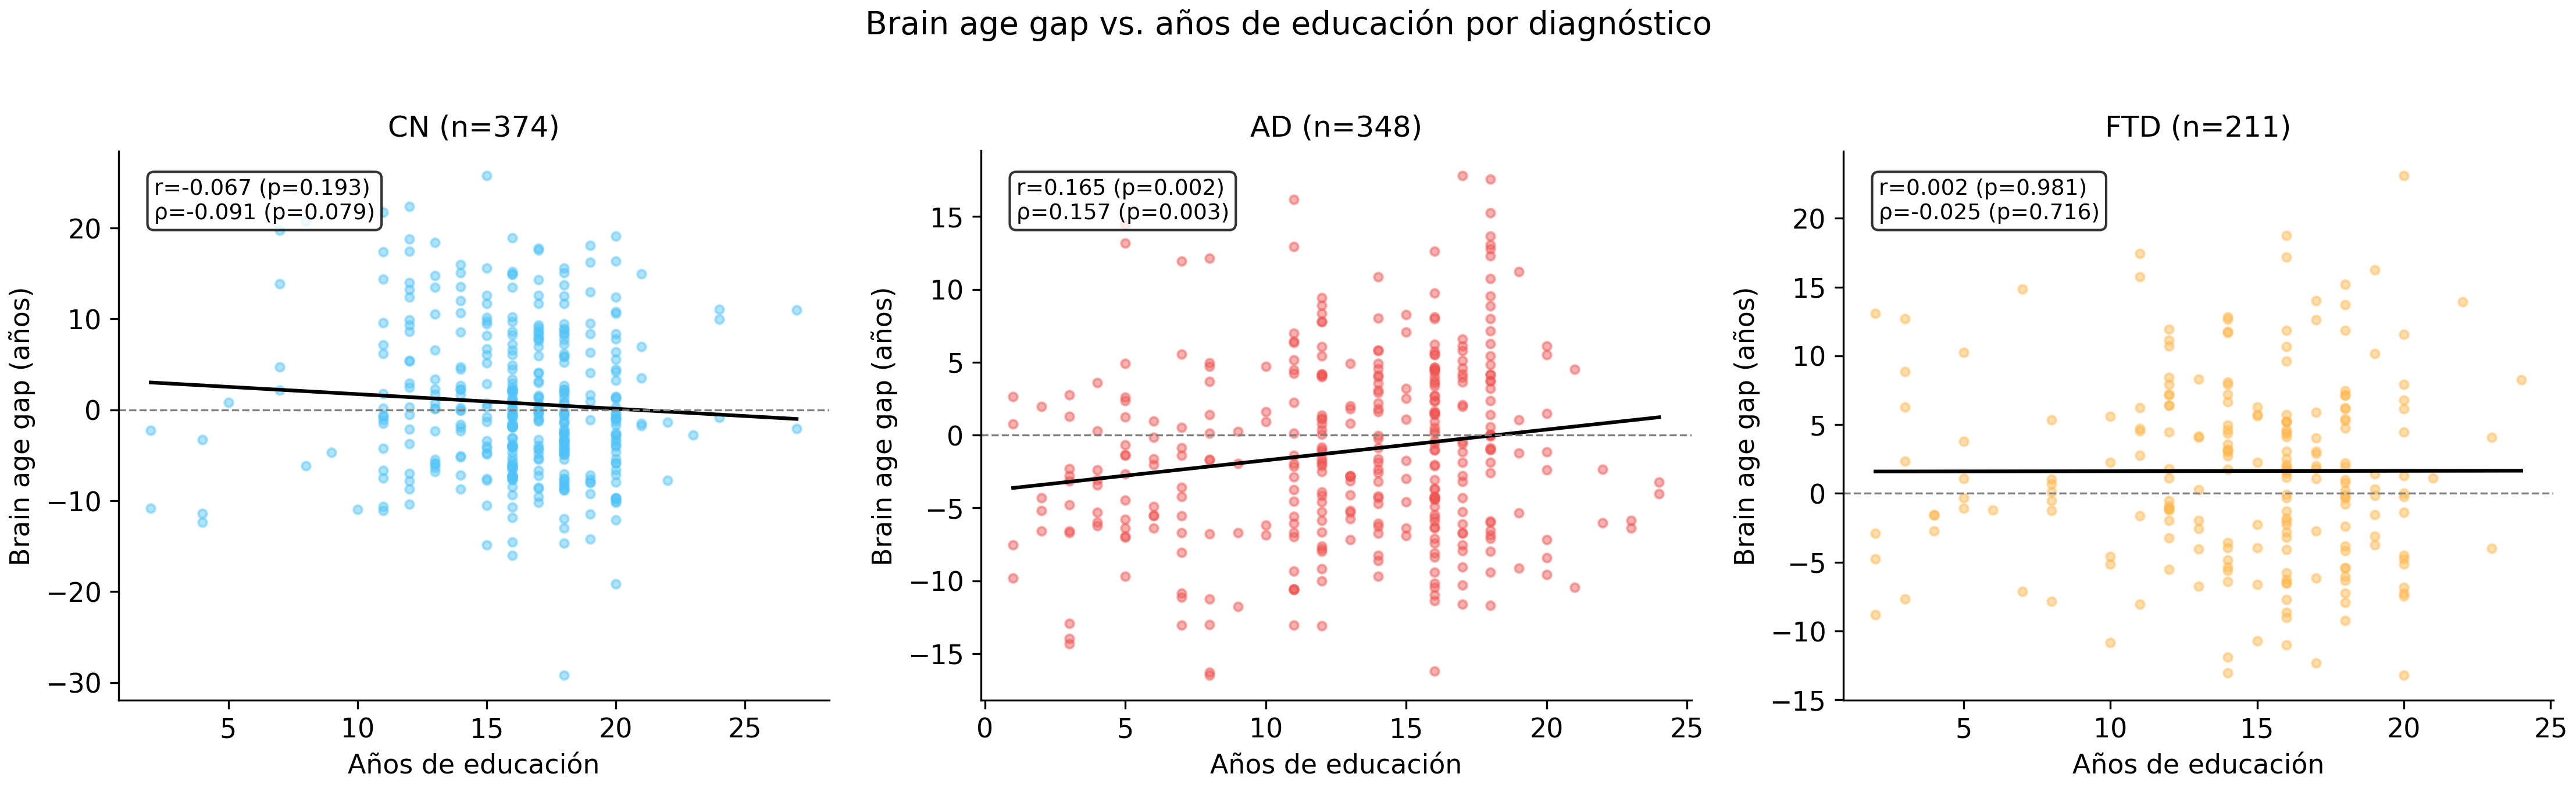
\includegraphics[width=0.95\textwidth]{06_resultados_discusion/images/demo_gap_vs_education.png}
\caption{Brain age gap vs.\ años de educación por grupo diagnóstico. La recta indica la tendencia lineal. En AD se observa una correlación positiva significativa; en CN una tendencia negativa débil; en FTD ausencia de correlación.}
\label{fig:demo_gap_vs_education}
\end{figure}

\subsection{Brain age gap y sitio de adquisición}
\label{sec:res_gap_sitio}

Con el fin de evaluar si los sujetos de distintos sitios de adquisición presentan brain age gaps distintas entre sí, o si las diferencias observadas podrían deberse al azar, se utilizó un análisis de varianza (\textbf{ANOVA}), una prueba estadística diseñada para comparar los promedios de tres o más grupos a la vez. La lógica de ANOVA es la siguiente: si todos los grupos tuvieran realmente la misma gap promedio, las diferencias que veríamos entre ellos serían pequeñas y comparables a la variación que existe dentro de cada grupo; en cambio, si las diferencias entre grupos son mucho mayores que la variación interna, ANOVA lo detecta con un valor $p$ bajo ($p < 0{,}05$), indicando que las diferencias son reales. En este caso, ANOVA arrojó $F = 8{,}67$ con $p < 0{,}001$, lo que confirma que el sitio de adquisición sí tiene un efecto significativo sobre la brain age gap.

La Tabla~\ref{tab:gap_site} presenta las estadísticas descriptivas de la gap por sitio para los sitios con al menos 20 sujetos. La columna ``gap media'' es el promedio de la brain age gap (edad predicha $-$ edad real) de los sujetos de cada sitio: por ejemplo, si un sitio tiene una gap media de $+4{,}30$ años, significa que en promedio el modelo predice que los cerebros de las personas de ese centro son 4,3 años más viejos de lo que realmente son. Un valor negativo indica lo contrario. La columna ``DE'' es la desviación estándar, que mide cuánta variación hay entre los sujetos de un mismo sitio.

\begin{table}[H]
\centering
\caption{Brain age gap por sitio de adquisición (sitios con $n \geq 20$). Se observan diferencias significativas entre sitios (ANOVA $p < 0{,}001$).}
\label{tab:gap_site}
\begin{tabular}{lrrr}
\toprule
\textbf{Sitio} & \textbf{$n$} & \textbf{Gap media} & \textbf{DE} \\
\midrule
Bruno       & 48  & $+$4,30 & 8,80 \\
Takada      & 89  & $+$2,82 & 9,20 \\
Slachevsky  & 93  & $+$1,15 & 7,89 \\
Matallana   & 135 & $+$0,92 & 6,21 \\
Miller      & 400 & $-$0,20 & 6,69 \\
Behrens     & 60  & $-$1,05 & 6,80 \\
Lopera      & 88  & $-$3,64 & 6,04 \\
\bottomrule
\end{tabular}
\end{table}

La Figura~\ref{fig:demo_gap_by_site} muestra la distribución de la brain age gap por sitio de adquisición.

\begin{figure}[H]
\centering
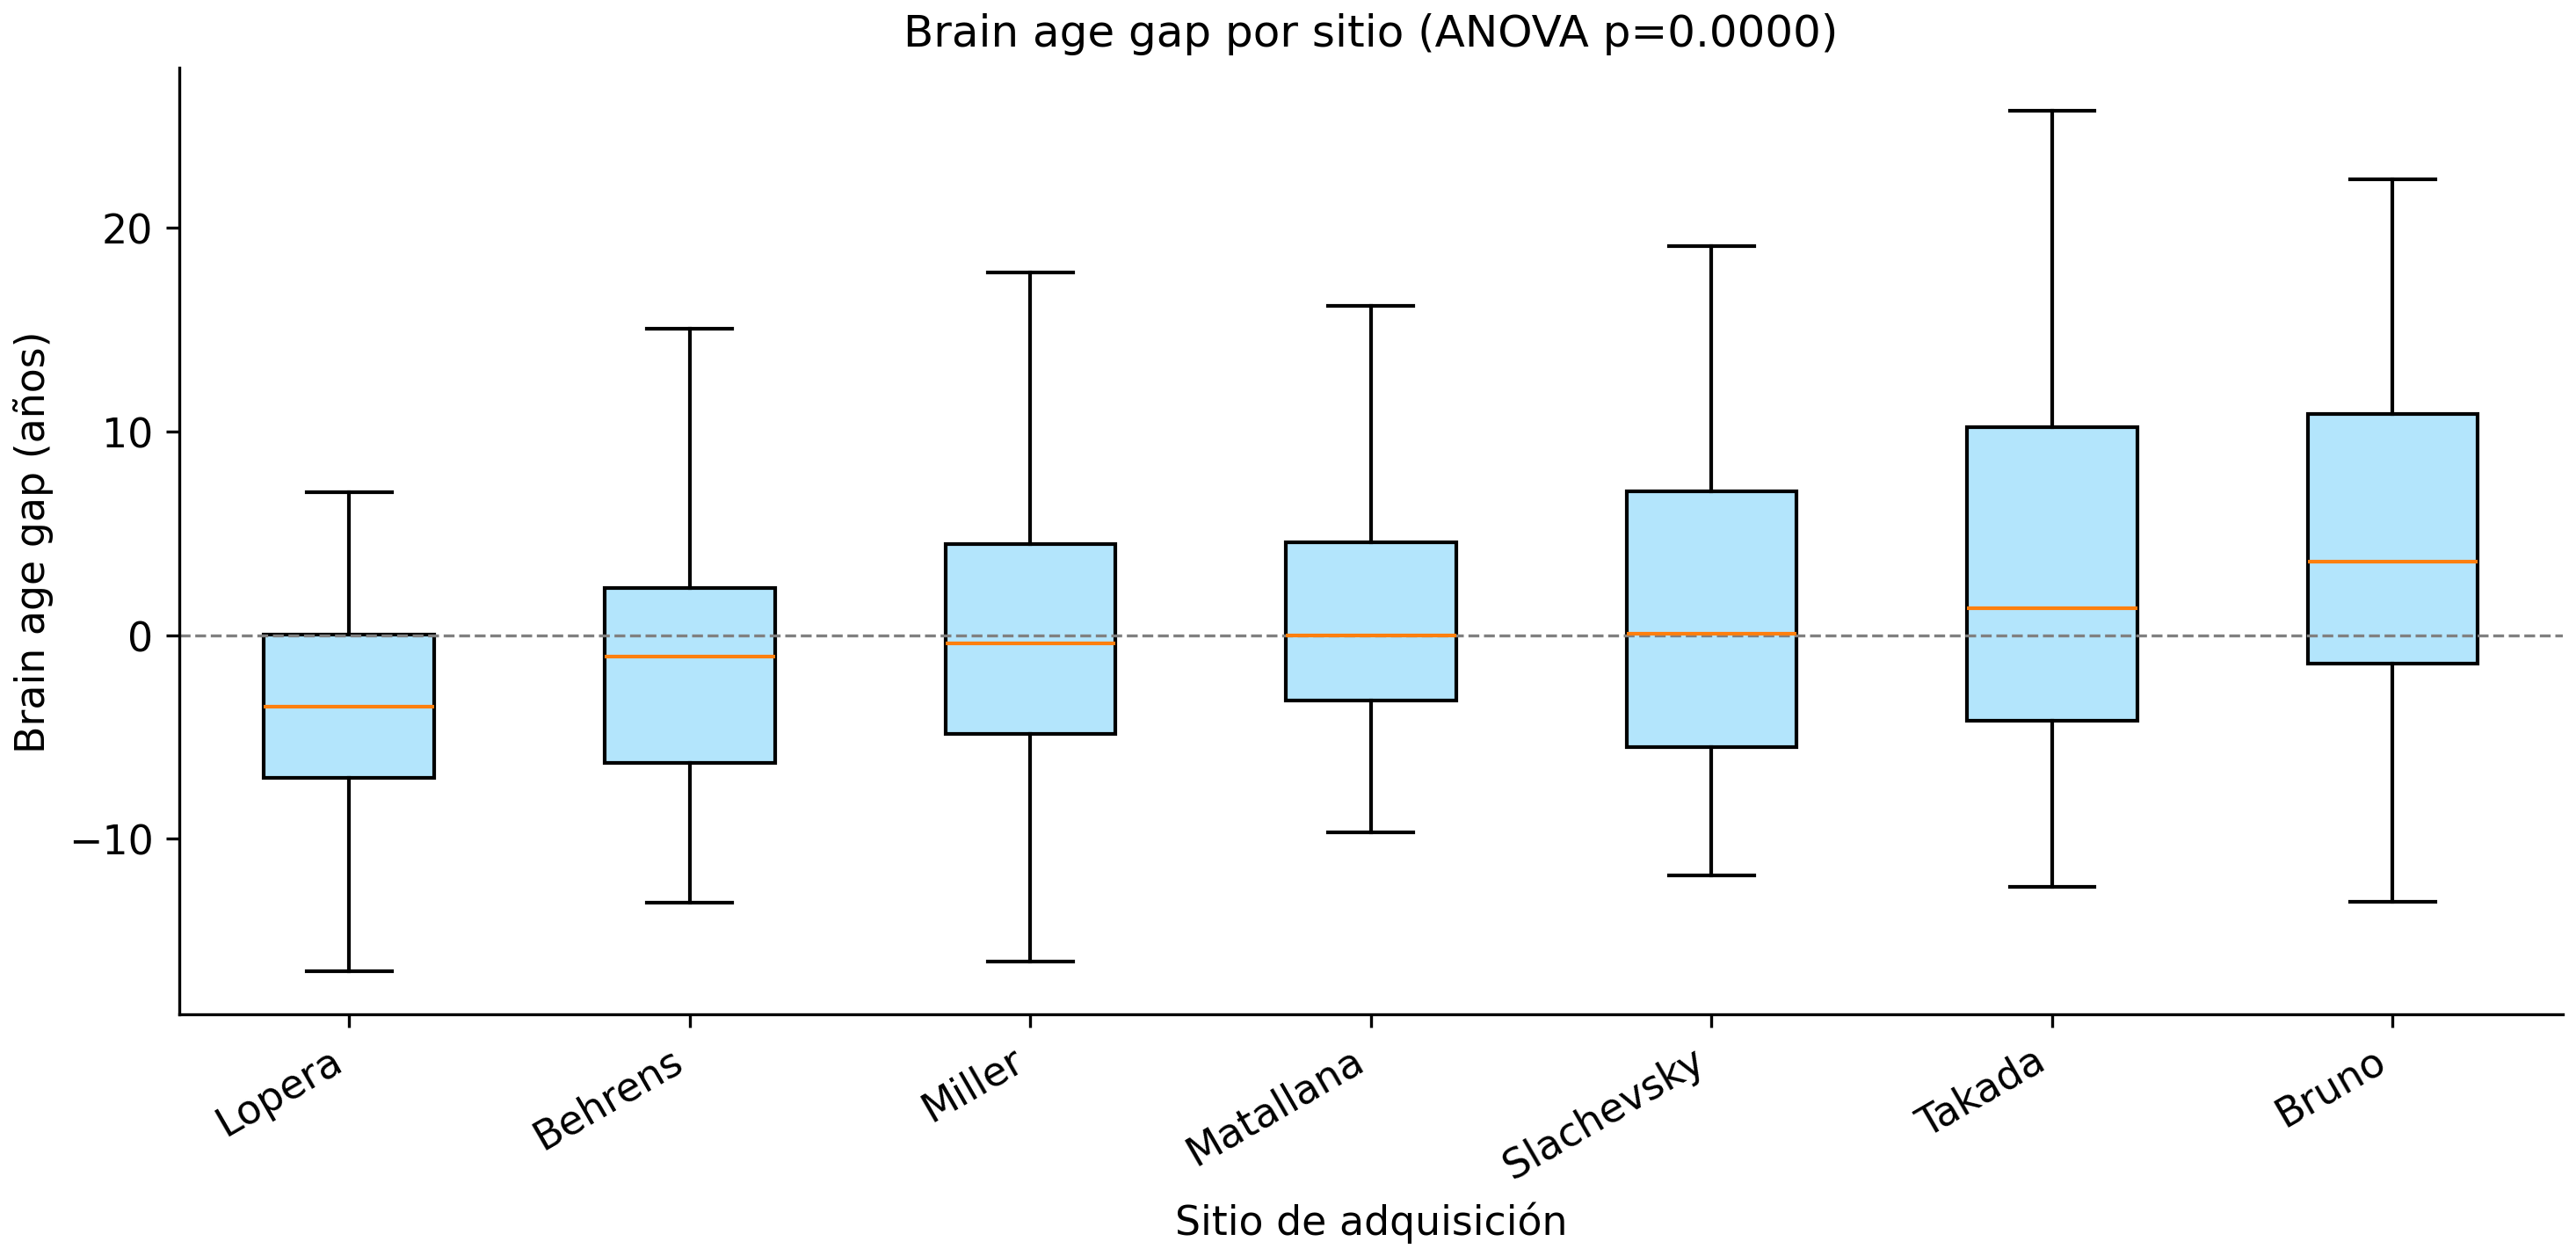
\includegraphics[width=0.85\textwidth]{06_resultados_discusion/images/demo_gap_by_site.png}
\caption{Distribución de la brain age gap por sitio de adquisición (sitios con $n \geq 20$). Las diferencias entre centros son estadísticamente significativas (ANOVA $p < 0{,}001$).}
\label{fig:demo_gap_by_site}
\end{figure}

La variabilidad entre sitios es considerable: la diferencia entre el sitio con mayor gap media (Bruno, $+4{,}30$ años) y el de menor (Lopera, $-3{,}64$ años) es de casi 8 años. Esta variabilidad inter-sitio refleja diferencias en los protocolos de adquisición, las características del escáner, la composición diagnóstica y las particularidades demográficas de cada centro. El análisis por marca de escáner reveló un patrón consistente: los sujetos adquiridos con escáneres Philips presentaron la gap media más alta ($+4{,}33$ años, $n = 47$ sujetos), seguidos por GE (gap media $+0{,}95$ años, $n = 289$) y Siemens (gap media $-0{,}26$ años, $n = 581$). Dado que Siemens concentra el 63\% de la muestra, el modelo aprendió predominantemente a partir de imágenes de esta marca; al recibir imágenes de Philips o GE, las diferencias técnicas entre escáneres pueden generar predicciones sistemáticamente sesgadas. Estos resultados subrayan la importancia de considerar técnicas de armonización entre sitios (como ComBat \cite{fortin2017harmonization}) en futuros trabajos con cohortes multicéntricas.

\subsection{Variables demográficas como features de predicción}
\label{sec:res_demo_ablacion}

Se evaluó si la inclusión de los años de educación y/o el sitio de adquisición como features adicionales mejora la predicción de edad. Para cada configuración, los hiperparámetros de XGBoost se optimizaron de forma independiente con Optuna (100 trials, 5-fold CV), garantizando que cada modelo disponga de parámetros ajustados a su espacio de features específico. Dado que estas variables no están disponibles para todos los sujetos, las configuraciones que las utilizan operan sobre una cohorte reducida. La Tabla~\ref{tab:demo_ablation} presenta los resultados.

\begin{table}[H]
\centering
\caption{Ablaciones con variables demográficas como features adicionales, cada una con hiperparámetros de XGBoost optimizados independientemente con Optuna. La reducción de $N$ se debe a la disponibilidad parcial de educación y sitio ($\sim$75\% de la cohorte). Se resalta en negrita la configuración con mejor MAE.}
\label{tab:demo_ablation}
\resizebox{\textwidth}{!}{%
\begin{tabular}{lrrrrrr}
\toprule
\textbf{Configuración} & \textbf{$n_{\text{train}}$} & \textbf{$n_{\text{test}}$} & \textbf{Features} & \textbf{MAE} & \textbf{$R^2$} & \textbf{Pearson} \\
\midrule
VAE + T1w                    & 1120 & 125 & 180 & 5,62 & 0,411 & 0,644 \\
VAE + T1w + educación        &  842 &  91 & 181 & 5,33 & 0,502 & 0,711 \\
VAE + T1w + sitio            &  848 &  93 & 189 & 5,37 & 0,538 & 0,744 \\
\textbf{VAE + T1w + edu + sitio} & \textbf{842} & \textbf{91} & \textbf{190} & \textbf{5,17} & \textbf{0,523} & \textbf{0,725} \\
\bottomrule
\end{tabular}}
\end{table}

La configuración que combina educación y sitio con hiperparámetros optimizados independientemente alcanza un MAE de 5,17 años, una mejora de 0,45 años respecto al baseline (5,62). Todas las configuraciones con variables demográficas superan al baseline en todas las métricas. La configuración con sitio obtiene el mejor $R^2$ (0,538), mientras que la combinación de educación y sitio logra el mejor MAE. Estos resultados deben interpretarse con cautela, ya que las configuraciones con demográficos operan sobre una cohorte reducida ($n_{\text{test}} = 91$--$93$ vs.~$125$) compuesta por los sujetos que disponen de los datos correspondientes; la diferencia en la composición del conjunto de test puede contribuir a parte de las diferencias observadas.

\subsubsection{Importancia de las variables demográficas en la predicción}

La Figura~\ref{fig:demo_importance} muestra las 20 features más importantes según XGBoost para las tres configuraciones con variables demográficas. En la configuración con educación únicamente, la variable \texttt{education} aparece entre las features más relevantes, lo que indica que el modelo aprovecha activamente esta información para refinar sus predicciones. En las configuraciones que incluyen sitio, las variables de sitio codificadas mediante one-hot (véase Sección~\ref{sec:demo_method}) también aparecen entre las features más importantes; en particular, \texttt{site\_Miller} ocupa consistentemente las primeras posiciones. La prominencia de \texttt{site\_Miller} se explica por su tamaño: con 400 sujetos, representa aproximadamente el 42\% de la subcohorte con información de sitio. El modelo aprende a reconocer las características propias de las imágenes de este centro (asociadas a su escáner, protocolo y población) y utiliza la variable binaria de sitio como un indicador que distingue ``imagen típica de Miller'' del resto, capturando así diferencias técnicas y demográficas sistemáticas. Que una sola variable categórica supere en importancia a muchas features de neuroimagen evidencia la magnitud de la variabilidad multicéntrica en la cohorte. En la configuración combinada (educación + sitio), ambas fuentes de información contribuyen de forma complementaria: las features de neuroimagen (T1w y embeddings del VAE) siguen dominando, pero las variables demográficas aportan señal adicional que reduce el error de predicción.

\begin{figure}[H]
\centering
\begin{subfigure}[b]{0.48\textwidth}
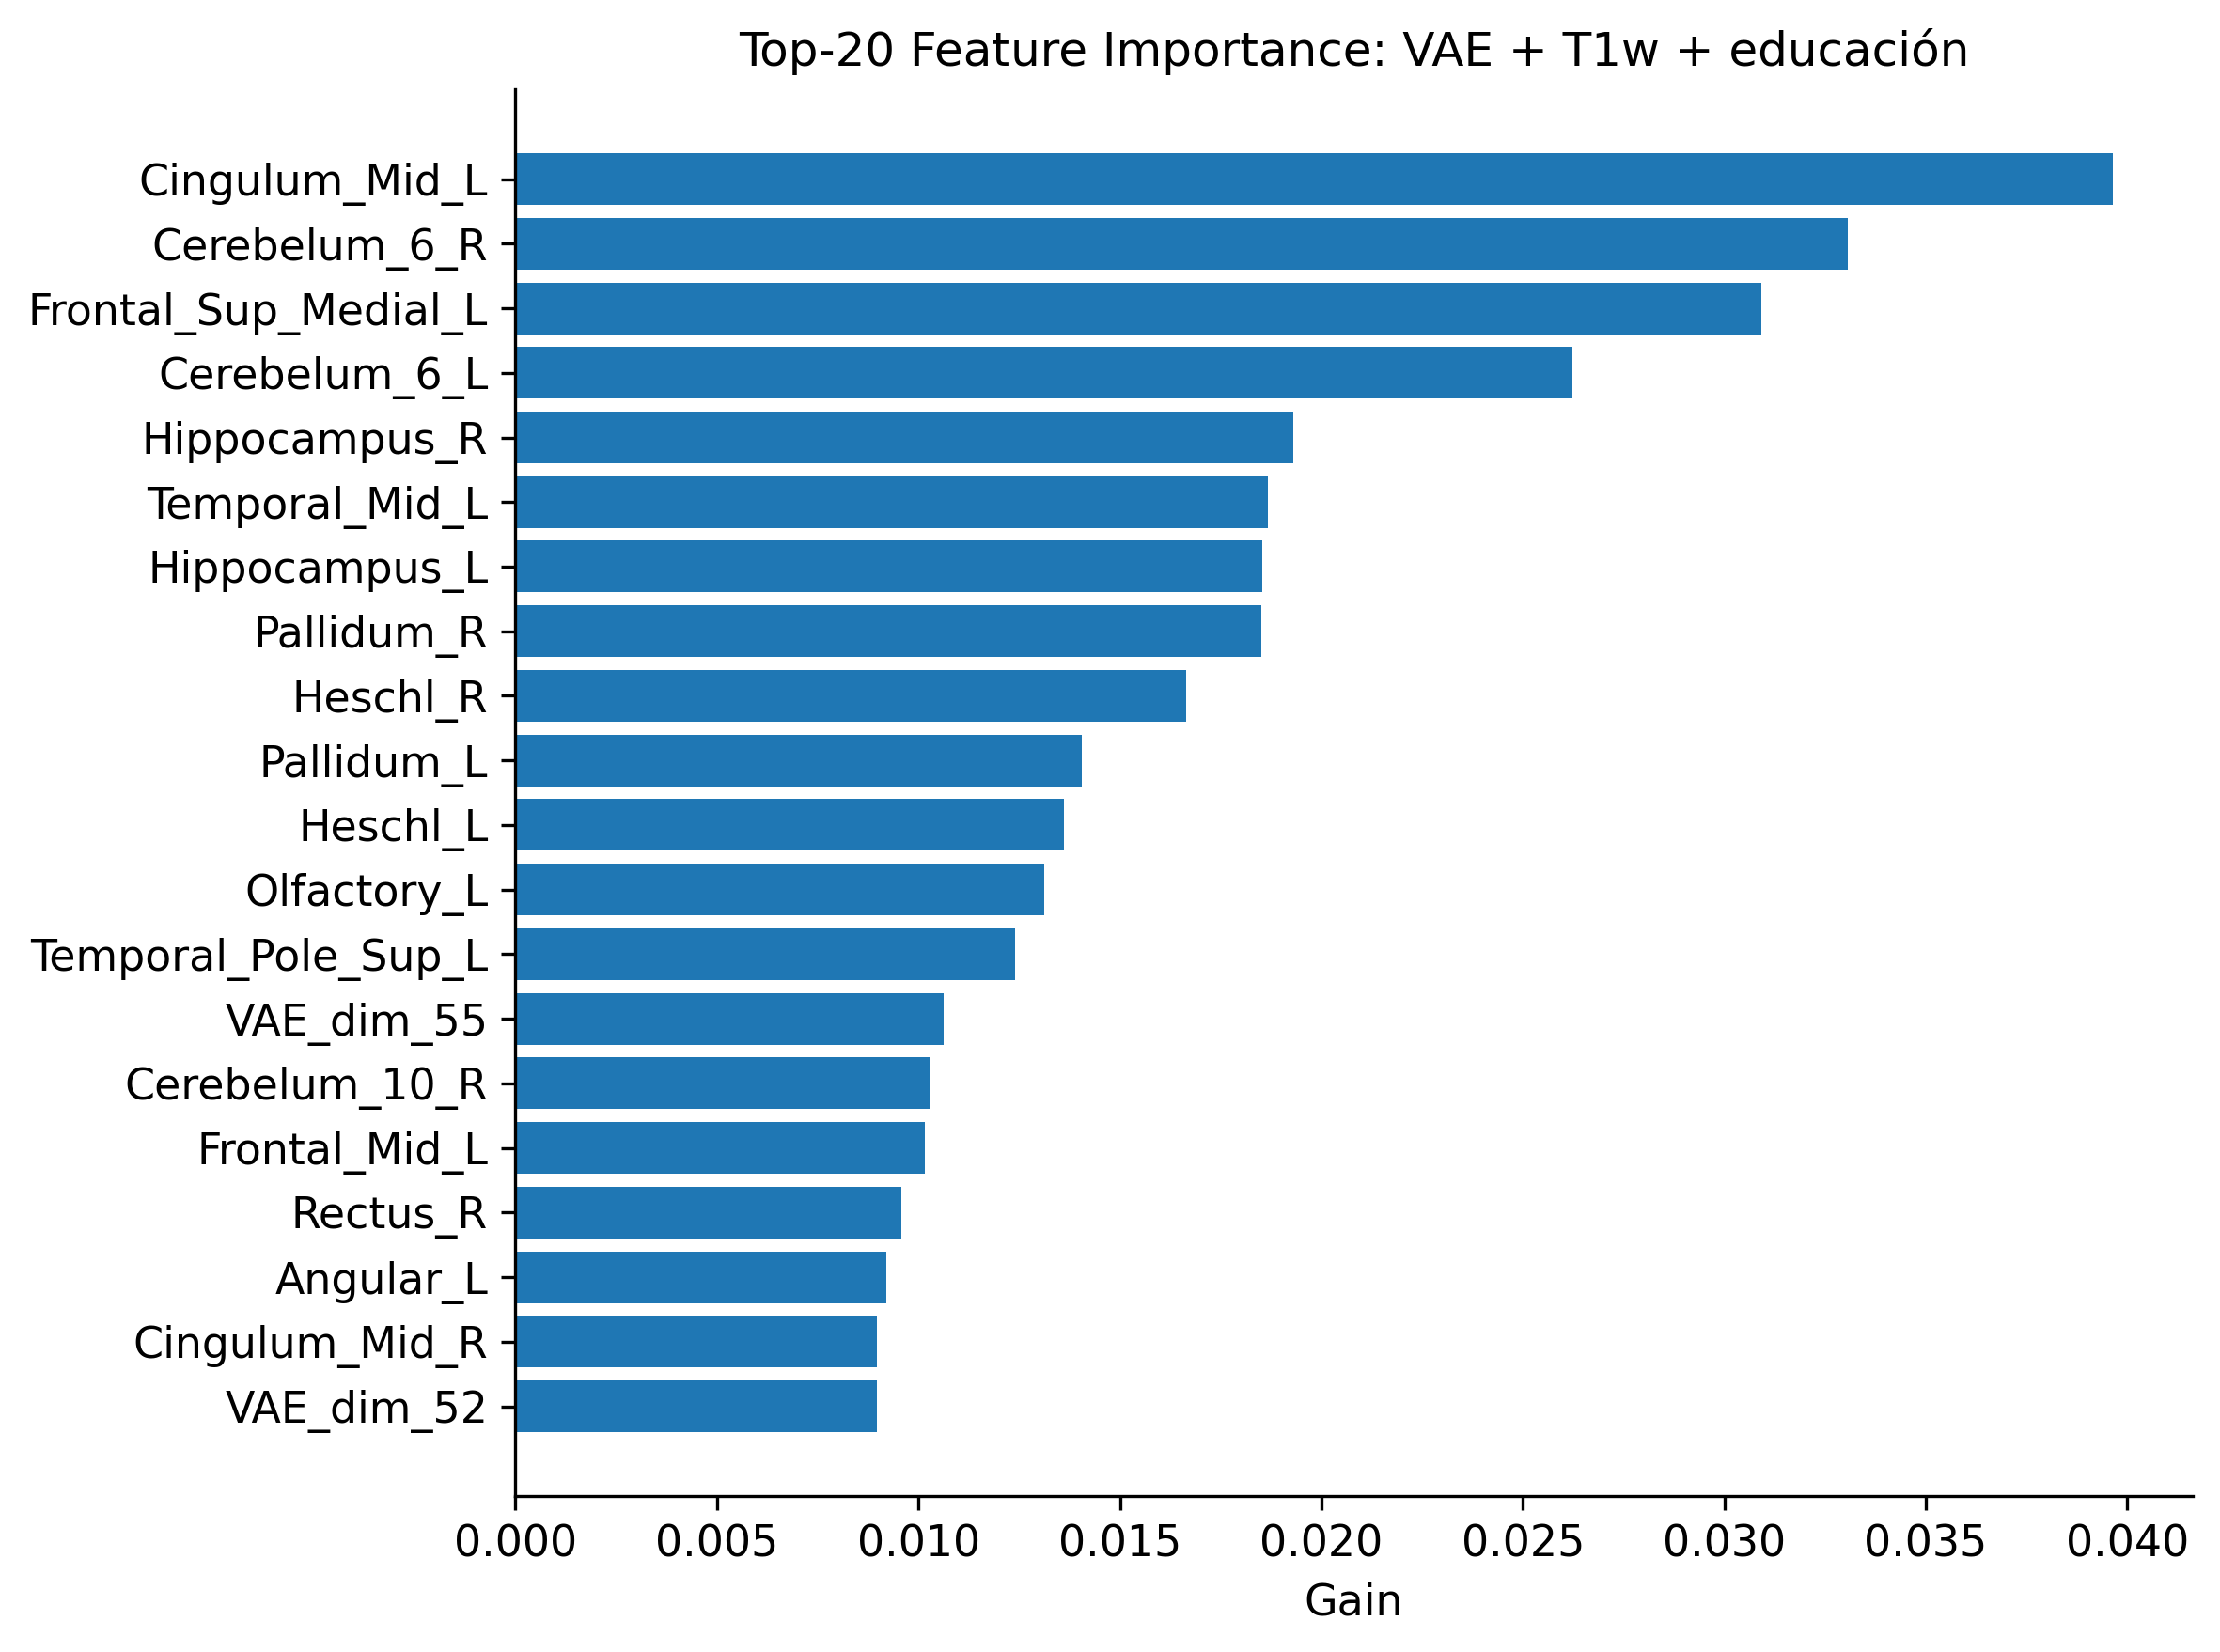
\includegraphics[width=\textwidth]{06_resultados_discusion/images/demo_importance_VAE__T1w__educacion.png}
\caption{VAE + T1w + educación}
\end{subfigure}
\hfill
\begin{subfigure}[b]{0.48\textwidth}
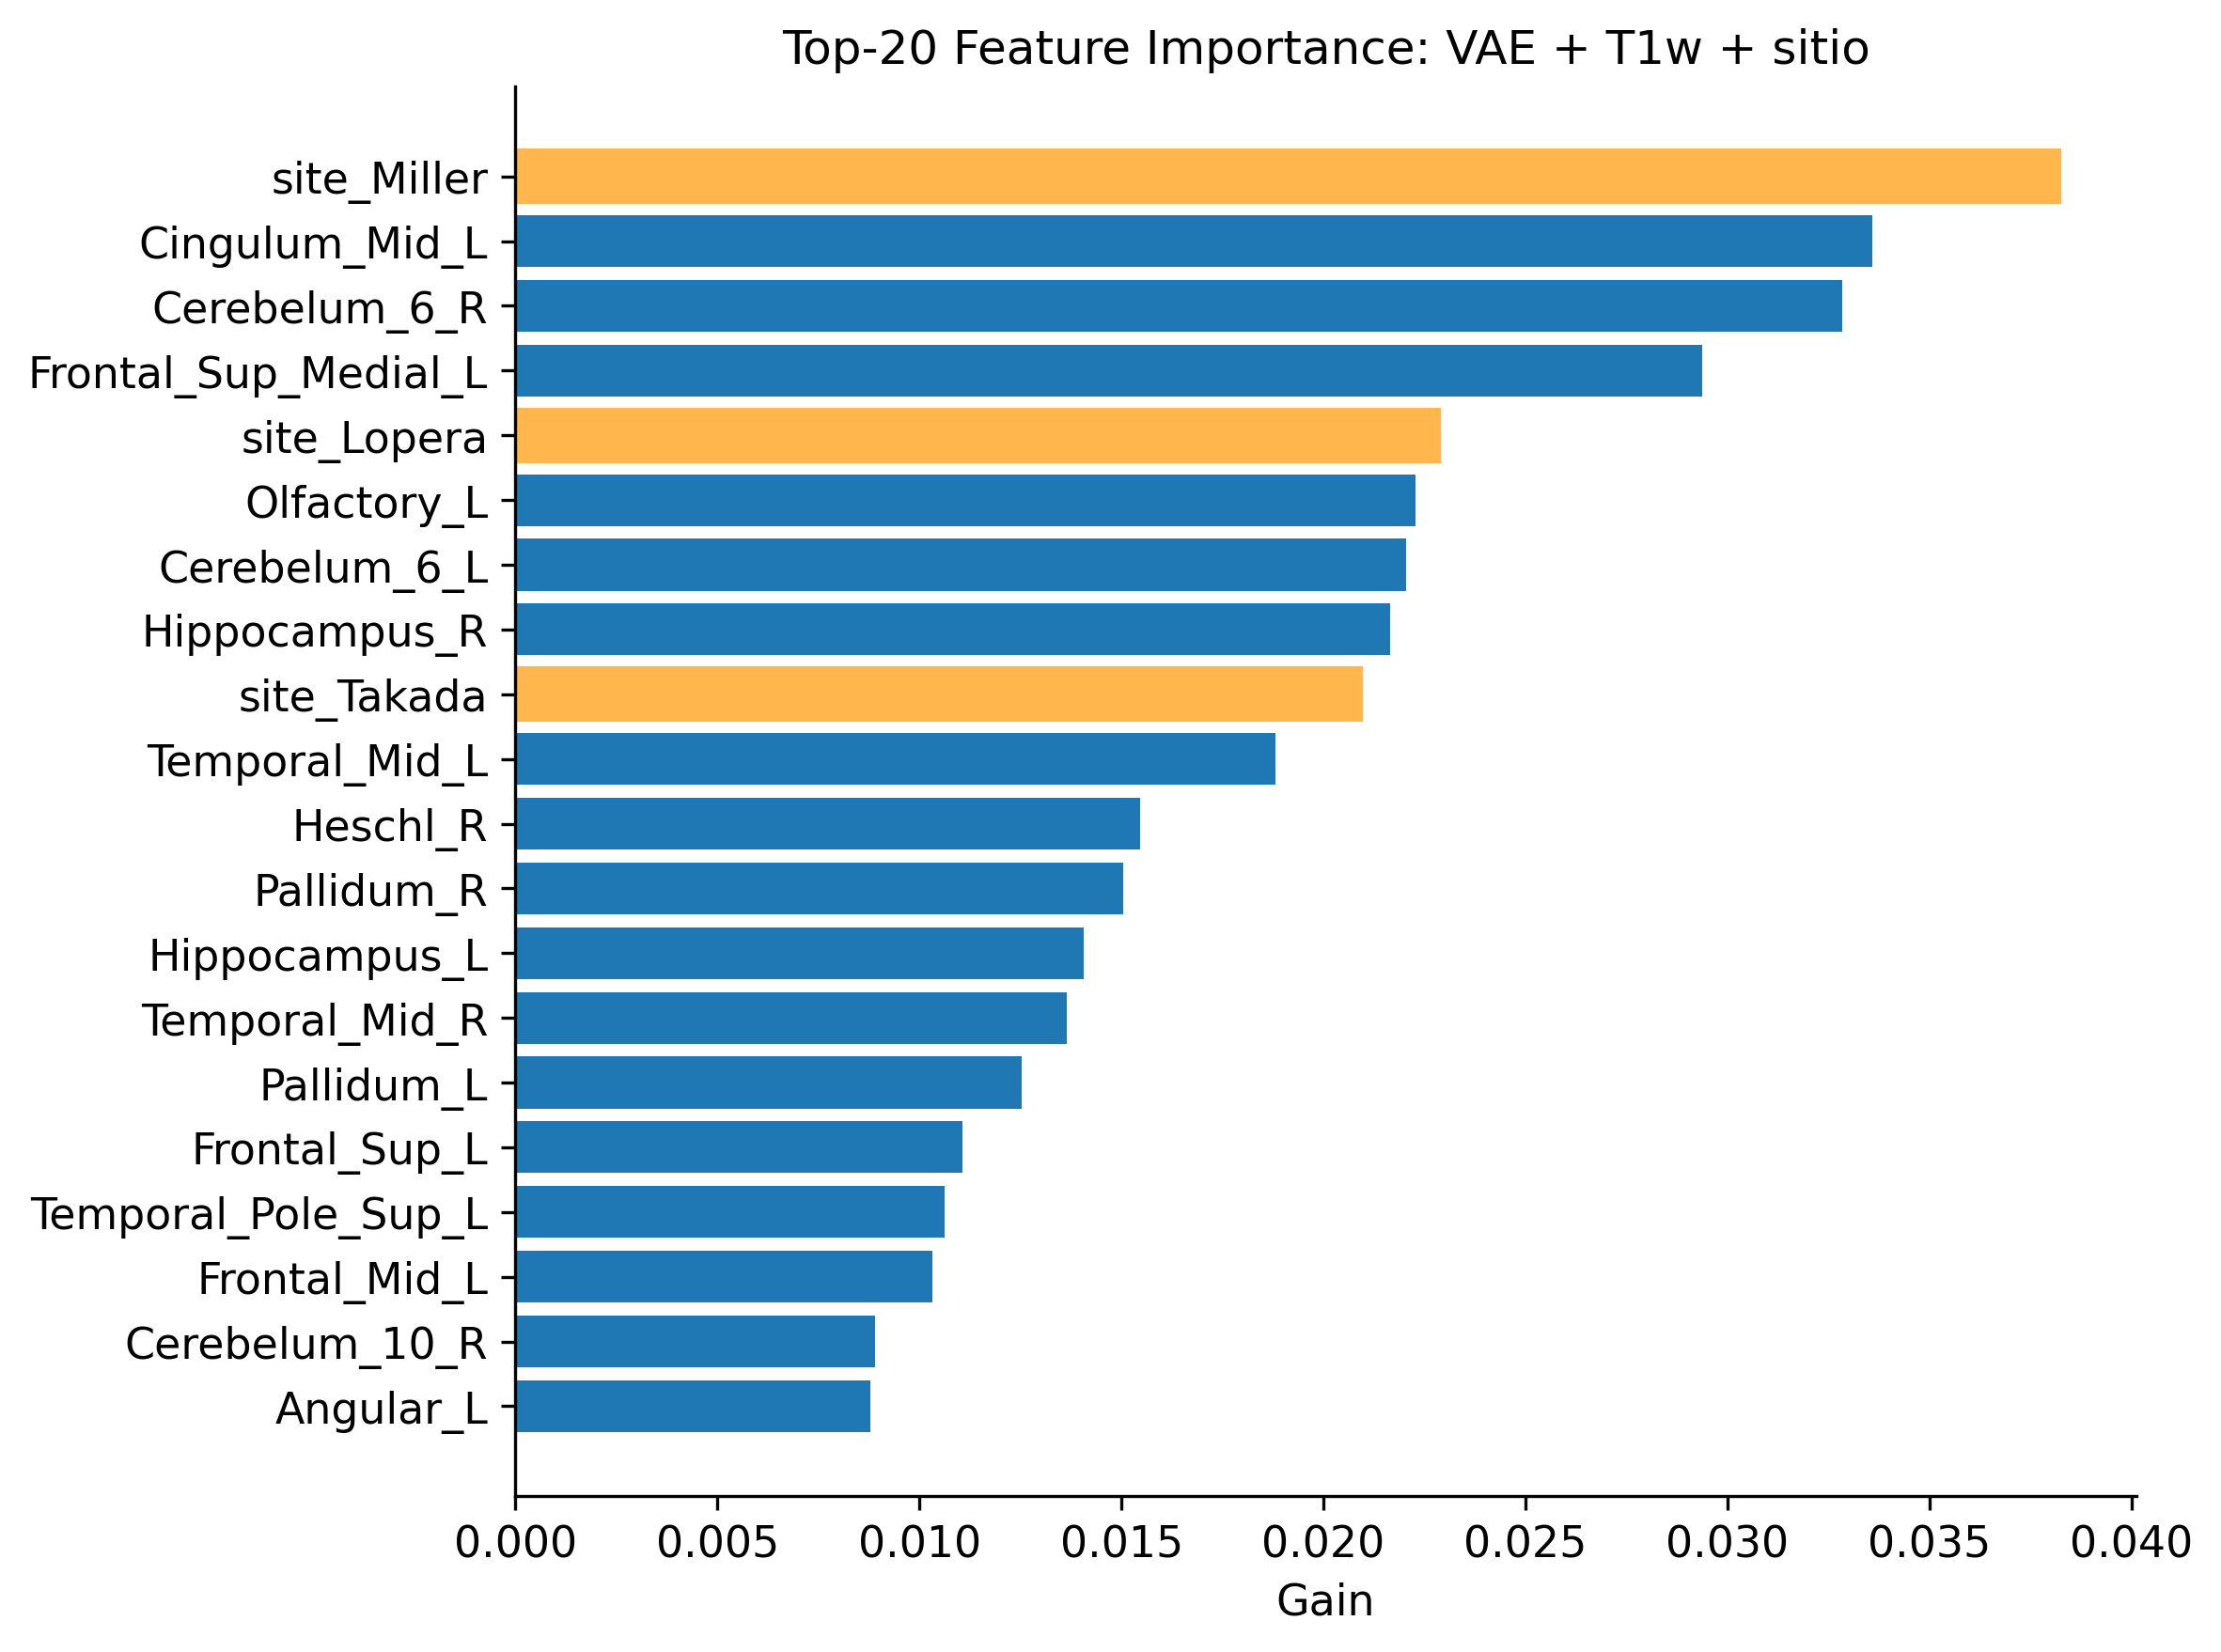
\includegraphics[width=\textwidth]{06_resultados_discusion/images/demo_importance_VAE__T1w__sitio.png}
\caption{VAE + T1w + sitio}
\end{subfigure}

\vspace{0.5cm}
\begin{subfigure}[b]{0.48\textwidth}
\centering
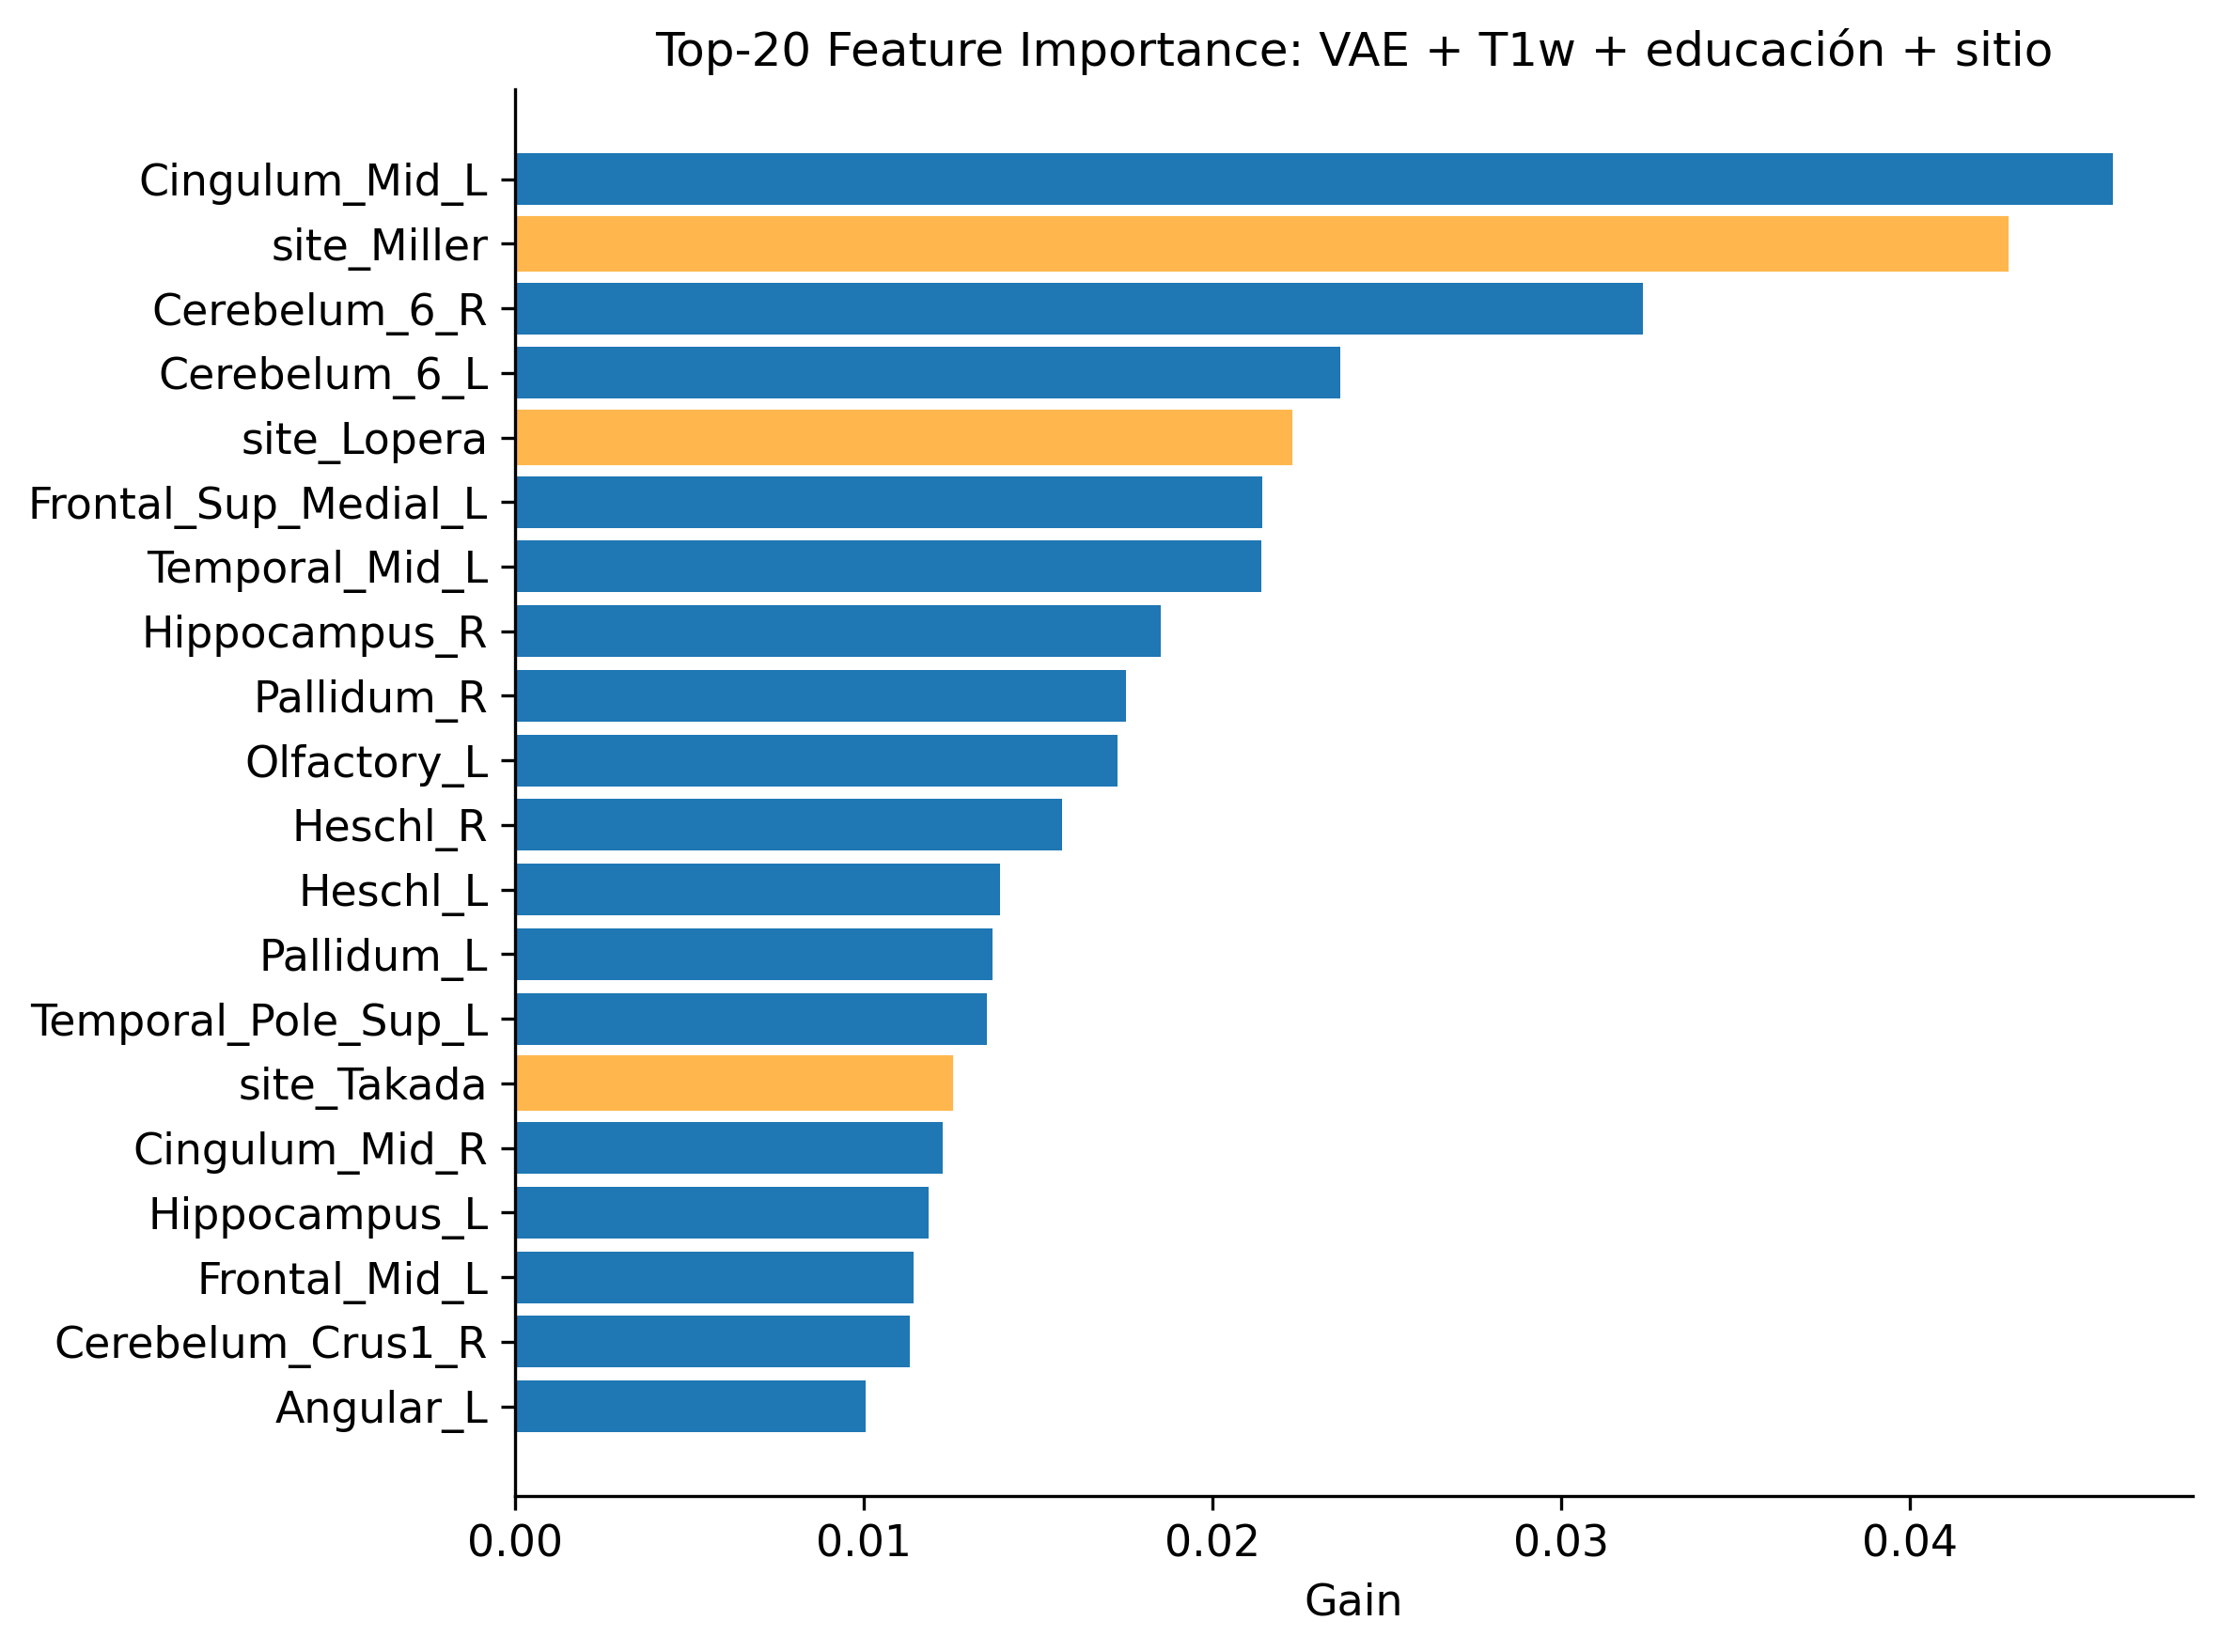
\includegraphics[width=\textwidth]{06_resultados_discusion/images/demo_importance_VAE__T1w__educacion__sitio.png}
\caption{VAE + T1w + educación + sitio}
\end{subfigure}
\caption{Top 20 features por importancia (XGBoost \textit{gain}) para cada configuración con variables demográficas. Las features con nombre anatómico (p.~ej.\ Cerebellum\_6\_R) corresponden a volúmenes T1w del atlas AAL-116. Las etiquetadas como VAE\_dim\_$N$ son dimensiones del espacio latente del $\beta$-VAE, que codifican patrones de conectividad funcional aprendidos de forma no supervisada; al no representar una región cerebral individual sino una combinación de conexiones, no admiten una interpretación anatómica directa. Las features demográficas (\texttt{education}, \texttt{site\_X}) aparecen entre las más relevantes junto con las de neuroimagen.}
\label{fig:demo_importance}
\end{figure}

Una regresión lineal de la brain age gap sobre las variables demográficas reveló que la educación por sí sola explica menos del 1\% de la varianza de la gap ($R^2 = 0{,}005$). Al agregar sexo y diagnóstico, la varianza explicada sube al 2,6\%, y al incluir el sitio alcanza el 8,0\%. La varianza explicada ($R^2$) indica qué porcentaje de la variabilidad total de la variable respuesta es capturado por el modelo: un $R^2 = 0{,}08$ (8\%) significa que las variables demográficas dan cuenta de solo el 8\% de las diferencias observadas en la brain age gap, mientras que el 92\% restante se debe a otros factores (diferencias neurobiológicas reales, ruido de medición, etc.). Esto confirma que el sitio de adquisición es el factor demográfico con mayor influencia sobre la gap, actuando como un confundidor que captura diferencias técnicas y poblacionales entre centros.


\section{Discusión}
\label{sec:discusion}

\subsection{Rendimiento en contexto e integración multimodal}

El modelo principal obtuvo un MAE de 5,62 años en el conjunto de test. Este resultado se encuentra dentro del rango típico reportado en la literatura de estimación de brain age, donde los estudios con datasets de tamaño comparable ($N \approx 1000\text{--}2000$) reportan valores de MAE entre 4 y 8 años \cite{franke2010estimating}. Los estudios basados en cohortes significativamente mayores ($N > 10\,000$), como UK Biobank, han alcanzado valores de MAE entre 2 y 4 años, beneficiándose de la mayor cantidad de datos y de la homogeneidad de los protocolos de adquisición. Es importante señalar que la mayoría de estos trabajos entrenan sus modelos exclusivamente sobre controles sanos, mientras que el presente pipeline fue entrenado sobre la cohorte completa (CN, AD y FTD). Entrenar con sujetos que presentan patologías neurodegenerativas introduce mayor heterogeneidad en los patrones de envejecimiento, lo que hace que el problema de regresión sea más difícil. Que el modelo alcance un MAE comparable al de estudios que solo entrenan con controles sanos sugiere que el pipeline logra capturar patrones generales de envejecimiento aun en presencia de esta variabilidad adicional. Por otro lado, la cohorte RedLaT integra datos de múltiples centros latinoamericanos con protocolos potencialmente heterogéneos, lo que introduce una fuente de ruido adicional y hace que la comparación directa con otros estudios deba interpretarse con cautela.

La combinación de conectividad funcional (vía $\beta$-VAE) con datos estructurales T1w mejora la predicción respecto al uso de cualquiera de las dos fuentes por separado: la mejora de 0,27 años en MAE y de 0,045 en $R^2$ al agregar los embeddings del VAE a T1w es consistente y se observa en todas las métricas. Al mismo tiempo, los embeddings por sí solos resultan insuficientes (MAE = 7,01), lo que sugiere que la conectividad funcional es una fuente de información más ruidosa que los datos estructurales y se beneficia de la complementación. La fusión a nivel de features permite que el regresor identifique las combinaciones más informativas de ambas fuentes.

La comparación entre regresores (Sección~\ref{sec:res_regresores}) refuerza esta observación: Ridge, SVR y XGBoost alcanzan prácticamente el mismo rendimiento (diferencia máxima de 0,13 años en MAE), lo que sugiere que, una vez construidas representaciones de calidad, la elección del regresor tiene un impacto marginal. Este resultado es coherente con la observación de que las features del VAE son suaves y continuas, un escenario favorable para distintas familias de modelos.

\subsection{Modelado no lineal y estrategias de entrenamiento}

Un resultado notable es la equivalencia práctica entre PCA y $\beta$-VAE como métodos de reducción de dimensionalidad (Sección~\ref{sec:res_pca}): ambos alcanzan un MAE $\approx$ 5,6 y un $R^2 \approx$ 0,42, con diferencias menores a 0,02 en todas las métricas. Esto sugiere que la información relevante para la predicción de edad en las matrices FC es capturada en buena medida por las direcciones de máxima varianza (componentes principales), y que un regresor potente como XGBoost puede extraer patrones no lineales incluso a partir de proyecciones lineales. Sin embargo, la reducción de dimensionalidad sí es necesaria: la comparación con features crudos de FC (Sección~\ref{sec:res_raw_fc}) muestra que, aun con hiperparámetros optimizados específicamente para la entrada de alta dimensionalidad, el pipeline sin compresión obtiene un MAE de 6,00 frente a 5,62 del pipeline comprimido, y un $R^2$ de 0,354 frente a 0,411. Es decir, el paso clave es la reducción de 6670 a 64 dimensiones, no el carácter lineal o no lineal de dicha reducción.

Es importante contextualizar la equivalencia PCA--VAE. La elección del $\beta$-VAE como componente del pipeline siguió la tendencia predominante en la literatura de neuroimagen, donde los autoencoders variacionales se han adoptado ampliamente para modelar datos cerebrales de alta dimensionalidad. La comparación con PCA fue realizada a posteriori como una validación de la necesidad de la complejidad no lineal del VAE. Además, la exploración del espacio de hiperparámetros del VAE fue necesariamente limitada: 70 trials de Optuna sobre un espacio combinatorio que incluye la dimensión latente, el número y tamaño de capas ocultas, $\beta$, dropout, learning rate, épocas de warmup y tipo de embedding. Con una exploración más exhaustiva o con técnicas de búsqueda más sofisticadas, el VAE podría potencialmente superar a PCA, especialmente a medida que el tamaño de la muestra aumente y las representaciones no lineales dispongan de más datos para capturar patrones sutiles. En cualquier caso, el resultado actual es informativo y consistente con los hallazgos de Monti et al.\ y More et al.\ discutidos en la Sección~\ref{sec:res_pca}. El presente trabajo extiende esas observaciones al mostrar que, para esta cohorte y esta dimensionalidad, la complejidad del VAE no aporta una ventaja mensurable en la predicción de edad, aunque sí ofrece capacidades adicionales (generación, reconstrucción) que un método puramente lineal no puede proporcionar.

En cuanto a la estrategia de entrenamiento, el modelo entrenado exclusivamente en controles sanos (Sección~\ref{sec:res_cn_only}) fue evaluado sobre la totalidad de los pacientes AD ($n = 422$) y FTD ($n = 297$), ya que ninguno de ellos fue utilizado durante el entrenamiento. A pesar de este mayor poder estadístico, los $R^2$ fueron negativos en ambos grupos clínicos, la brain age gap mostró una dirección inconsistente entre AD ($-1{,}86$~años) y FTD ($+1{,}84$~años), y las correlaciones de Pearson fueron inferiores a 0,2. Esto indica que, con $N = 473$ sujetos CN, el modelo no logra aprender la relación entre neuroimagen y edad con la precisión suficiente para que las desviaciones de esa norma constituyan un biomarcador confiable. Este resultado no invalida la estrategia CN-only en general, pero sugiere que requiere cohortes considerablemente mayores \cite{smith2019estimation}.

Resulta alentador, no obstante, que el modelo CN-only entrenado con variables demográficas (Sección~\ref{sec:res_cn_demo}) ---aun con solo 337 sujetos CN--- produce gaps consistentemente positivas en ambos grupos clínicos (AD: $+0{,}70$; FTD: $+4{,}11$), la dirección esperada en neurodegeneración. Aunque el tamaño de muestra es insuficiente para extraer conclusiones definitivas, este resultado sugiere que la inclusión de información demográfica podría facilitar la construcción de un biomarcador de envejecimiento cerebral cuando se disponga de cohortes CN más amplias.

\subsection{Variables demográficas y variabilidad multicéntrica}

El análisis del impacto de variables demográficas (Sección~\ref{sec:res_demograficas}) reveló que el sitio de adquisición es el factor con mayor influencia sobre la brain age gap, explicando el 8\% de su varianza cuando se combina con educación, sexo y diagnóstico. Las diferencias entre sitios alcanzan casi 8 años de gap media, lo que pone de manifiesto la necesidad de técnicas de armonización en cohortes multicéntricas. En la cohorte RedLaT, esta variabilidad inter-sitio refleja no solo diferencias técnicas (escáneres, protocolos) sino también diferencias poblacionales propias de cada centro latinoamericano.

Al incorporar la educación y el sitio como features adicionales del modelo con hiperparámetros optimizados independientemente mediante Optuna (Sección~\ref{sec:res_demo_ablacion}), se obtuvo un MAE de 5,17 años, la mejor configuración evaluada en este trabajo. Este resultado indica que las variables demográficas contienen información predictiva sobre la edad que no está completamente capturada por las features de neuroimagen. El análisis de importancia de features confirmó que tanto la educación como las variables de sitio se posicionan entre las features más relevantes del modelo, aportando señal complementaria a los embeddings del VAE y los volumenes T1w.

La educación, utilizada como indicador del nivel socioeconómico, mostró una correlación significativa con la gap únicamente en pacientes con AD ($r = +0{,}165$, $p = 0{,}002$). La dirección positiva (más educación $\rightarrow$ gap más alta) podría explicarse por un efecto de reserva cognitiva: los pacientes con mayor educación mantienen el funcionamiento cognitivo durante más tiempo, accediendo al diagnóstico en estadios más avanzados de la neurodegeneración, cuando la atrofia cerebral es más pronunciada. En controles sanos, la tendencia negativa ($r = -0{,}067$, no significativa) es consistente con la hipótesis de que la educación ejerce un efecto neuroprotector, aunque la señal es demasiado débil para alcanzar significancia con esta muestra. Estos resultados son relevantes en el contexto latinoamericano, donde la variabilidad en los niveles educativos es considerable y puede modular tanto el acceso al diagnóstico como la expresión clínica de la neurodegeneración.

\subsection{Limitaciones}
\label{sec:limitaciones}

El trabajo presenta varias limitaciones que conviene considerar. La más relevante es el tamaño de la cohorte: con $N = 1245$ sujetos, el dataset es significativamente menor que los empleados en estudios de referencia, lo que limita tanto la capacidad de generalización como el rendimiento del modelo (reflejado en un $R^2$ moderado de 0,411). Relacionado con esto, el modelo entrenado solo en CN mostró señales inconsistentes al evaluar la brain age gap en las poblaciones clínicas, lo que impidió su uso como biomarcador confiable. Los resultados exploratorios con variables demográficas en el modelo CN-only son prometedores (gaps positivas en AD y FTD), pero se basan en solo 337 sujetos de entrenamiento y requieren validación con cohortes más amplias.

El análisis de variables demográficas se limitó a las disponibles en la cohorte con cobertura suficiente (educación, sitio y marca de escáner). Otras variables de interés ---como el nivel de ingreso, la ocupación o el estatus socioeconómico--- no estaban disponibles o presentaban una cobertura insuficiente, lo que impidió un análisis más exhaustivo de los factores sociodemográficos que podrían modular el envejecimiento cerebral en poblaciones latinoamericanas.

Desde el punto de vista metodológico, se utilizó el atlas AAL con 116 regiones, que es una parcellación relativamente gruesa. Sería interesante evaluar el pipeline con atlas de mayor resolución, como el de Schaefer et al.\ \cite{schaefer2018local} (disponible con 100 a 1000 parcelas), que podrían capturar patrones más finos de conectividad funcional, aunque su impacto sobre la predicción de edad no está garantizado y requeriría una evaluación empírica. Además, no se aplicaron técnicas de armonización entre sitios (como ComBat \cite{fortin2017harmonization}) para reducir la variabilidad introducida por los diferentes protocolos de adquisición de los centros de RedLaT.

En relación con la optimización del VAE, la búsqueda de hiperparámetros mediante Optuna exploró 70 configuraciones de un espacio combinatorio extenso. Si bien el número de trials es razonable dado el costo computacional de entrenar cada VAE, representa una fracción pequeña del espacio total. Esta exploración limitada podría explicar en parte la equivalencia observada con PCA: no puede descartarse que una configuración del VAE no explorada hubiera producido representaciones superiores a las componentes principales.

Por último, el pipeline utiliza un enfoque en dos etapas donde el VAE y el XGBoost se optimizan de forma separada. Arquitecturas de deep learning end-to-end, como redes de grafos sobre matrices de conectividad o redes convolucionales 3D sobre volúmenes T1w, podrían integrar ambas etapas y potencialmente mejorar el rendimiento, aunque requieren muestras mayores para entrenarse de forma efectiva.